\documentclass[12pt, twoside, italian]{book}
\input{preamble/preamble}
\input{preamble/letterfonts}
\input{preamble/macros}
\usepackage{fancyhdr}
\usepackage{titlesec}  % Opzionale, per controllo avanzato sui titoli
\usetikzlibrary{arrows.meta, shapes.geometric, calc}
\setlength{\parindent}{0pt}
\setlength{\parskip}{0pt}
\pagestyle{fancy}

% Definizione dell'intestazione per pagine dispari (Odd)
\fancyhead[LO]{\textbf{\thepage}}  % Numero di pagina in grassetto a sinistra
\fancyhead[RO]{\nouppercase\rightmark}         % Capitolo e sezione a destra

% Definizione dell'intestazione per pagine pari (Even)
\fancyhead[LE]{\nouppercase\leftmark}          % Capitolo e sezione a sinistra
\fancyhead[RE]{\textbf{\thepage}}  % Numero di pagina in grassetto a destra

% Cancella il footer
\fancyfoot{}
\setlength{\headheight}{14.49998pt}
\addtolength{\topmargin}{-2.49998pt}
% Personalizzazione della linea orizzontale
\renewcommand{\headrulewidth}{0.4pt}
\renewcommand{\footrulewidth}{0pt}

\pgfplotsset{compat=newest}
\title{Appunti di teoria dei gruppi per la Fisica}
\author{Francesco Sermi}
\date{\today}
\pgfplotsset{
	compat = newest,
	colormap/violet % se si vuole cambiare il colormap utilizzato per generare i grafici, tuttavia la copertina ha un colormap a
					% parte che va modificato qua sotto. Se si stampa non a colori consiglio blackwhite come colormap
	}
\renewcommand{\appendixpage}{}
\begin{document}
	\begin{titlepage}
	\centering
	\vspace*{3cm}
	{\huge\bfseries Appunti di teoria dei gruppi per la Fisica \par}
	\vspace{2cm}
	{\Large\itshape Francesco Sermi\par}
	\vfill
	\begin{figure}[H]
		\centering
		%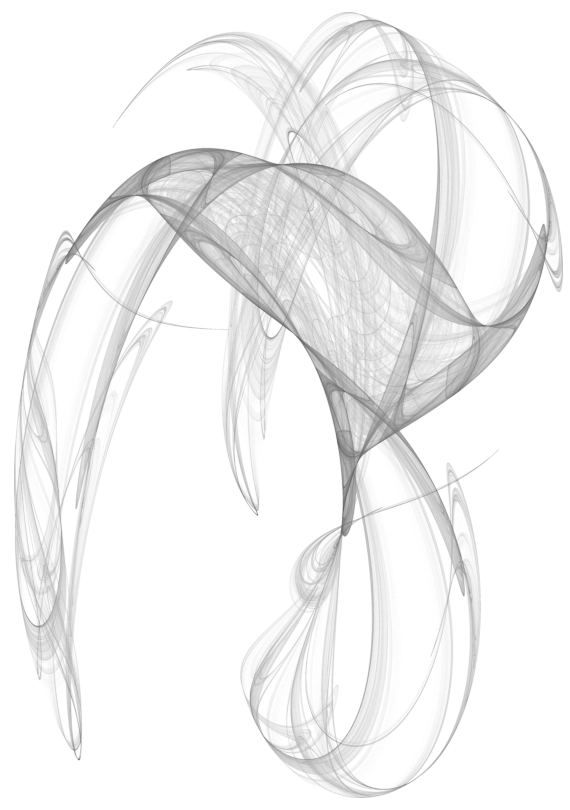
\includegraphics[width=0.65\textwidth]{immagini/dejong.png}
	\end{figure}
    	%\begin{tikzpicture}
	% Definisco lo stile dei vettori
    	%\tikzset{vector/.style={-stealth, thick, color=black}}

    % Parametri per il punto di contatto
    	%\def\xo{1}
    	%\def\yo{2}
    	%\def\zo{5} % Calcola z0 = f(x0, y0)

    % Derivate parziali della funzione f(x, y) = x^2 + y^2 nel punto (x0, y0)
    	%\def\fx{2*\xo} % = 2
    	%\def\fy{2*\yo} % = 4

    % Disegno la superficie
    	%\begin{axis}[
    	%    width=12cm,
    	%    view={60}{30}, % Angolazione impostata
    	%    axis lines=middle,
    	%    zlabel={$f(x,y)$},
    	%    clip=false,
    	%    domain=-5:5,
    	%    y domain=-5:5,
    	%    samples=30,
    	%    colormap/viridis,
    	%    z buffer=sort
    	%]

    % Grafico della superficie con colore visibile
    	%\addplot3[surf, opacity=0.8, shader=interp]
    	%    {x^2 - y^2}; % Superficie f(x, y) = x^2 + y^2
    	%\end{axis}
	%\end{tikzpicture}
	\vfill	
	\end{titlepage}
	\pagestyle{empty}
	%\vspace*{\fill}
    %Appunti di Geometria e Algebra Lineare  © 2025 by Francesco Sermi is licensed under Creative Commons Attribution-NonCommercial-NoDerivatives 4.0 International. To view a copy of this license, visit https://creativecommons.org/licenses/by-nc-nd/4.0/
	\cleardoublepage
	\vspace*{8cm}
	\begin{flushright}
    \begin{minipage}{0.65\textwidth}
        \itshape\small
        \noindent A mia madre. \\
    \end{minipage}
	\end{flushright}
	\cleardoublepage
	\pagestyle{fancy}
	\tableofcontents
	\chapter*{Introduzione}
	\pagestyle{empty}
	\thispagestyle{empty}
	\addcontentsline{toc}{chapter}{Introduzione}
	\markboth{Introduzione}{Introduzione}
	\pagestyle{fancy}
	Questi appunti nascono per riscrivere in forma pulita i miei appunti ed esercizi svolti di teoria dei gruppi, tenuto dal professore Kenichi Konishi nell'anno 2025/2026. In caso di errori, scrivetemi presso
	\begin{center}
		francesco291104 (\textbf{dot}) gmail.com
	\end{center}

	Buono studio a tutti! \\ \\ \\ \\
	\emph{Pisa, \today} \hfill Francesco Sermi\
	\vfill
	\cleardoublepage
	\chapter*{Notazioni}
	\markboth{Notazioni}{Notazioni}
	\pagestyle{empty}
	\thispagestyle{empty}
	\pagestyle{fancy}

	Riporto all'inizio del libro le notazioni adottate all'interno di questo documento (se non specificate dal contesto):
 	\begin{itemize}
		\item $(G, \circ)$ gruppo rispetto all'operazione $\circ$
		\item $e$ elemento identità di un gruppo
		\item $\sim$ relazione d'equivalenza
	\end{itemize}
	\newpage
	\chapter{Introduzione ai gruppi}

Lo scopo di questo capitolo è quello di introdurre il concetto di gruppo, mostrando alcuni esempi espliciti di gruppo, introducendone gli assiomi. La teoria dei gruppi, nonostante la sua applicazione alla Fisica sia piuttosto moderna, riveste un ruolo fondamentale, in quanto rappresenta il linguaggio naturale delle simmetrie dei sistemi fisici, classici e non, che incontriamo tutti i giorni.

\section{Assiomi di gruppo e teoria degli insiemi}

Se volessimo definire formalmente un gruppo, potremmo dare la seguente definizione

\begin{definition}[gruppo]
	Sia $G$ un insieme e sia $\cdot: G \times G \to G$ un'operazione, che chiameremo \emph{prodotto} che possiede le seguenti proprietà:
	\begin{enumerate}
		\item $\forall g_1, g_2 \in G, \exists g_3 \in G : g_1 \cdot g_2 = g_3$;
		\item $\forall g_1, g_2, g_3 \in G, g_1 \cdot (g_2 \cdot g_3) = (g_1 \cdot g_2) \cdot g_3$ (proprietà associativa);
		\item $\exists e \in G: \forall g \in G, e \cdot g = g$ (esistenza dell'elemento neutro);
		\item $\forall g \in G, \exists g^{-1} \in G: g^{-1} \cdot g = e$ (esistenza dell'elemento inverso);
	\end{enumerate}
\end{definition}

Da questi assiomi discendono le seguenti proprietà
\begin{prop}
	Se $(G, \cdot)$ è un gruppo, allora
	\begin{equation}
	\forall g \in G, g^{-1} \cdot g = g \cdot g^{-1} = e. 
	\end{equation}
\end{prop}
\begin{proof}
	Preso $g \in G$, sappiamo che $g^{-1} \cdot g = e$, in virtù dell'assioma $\circled{3}$, dunque sappiamo che, in virtù dell'assioma $\circled{4}$, possiamo moltiplicare a sinistra entrambi i lati per
	l'elemento inverso di $g^{-1}$, da cui 
	\begin{align}
	&g^{-1} \cdot g = e \implies (g^{-1})^{-1} \cdot g^{-1} \cdot g = (g^{-1})^{-1} \cdot e
	\end{align}
	e moltiplichiamo a destra entrambi i lati per $g^{-1}$ così da ottenere l'espressione di cui stiamo cercando il valore, ottenendo che
	\begin{align}
	&(g^{-1})^{-1} \cdot g^{-1} \cdot g \cdot g^{-1} = (g^{-1})^{-1} \cdot e \cdot g^{-1}\\
	\end{align}
	e a questo punto usiamo l'assioma $\circled{3}$ e l'assioma $\circled{4}$ per concludere che
	\begin{align}
	&e \cdot g \cdot g^{-1} = e \implies g \cdot g^{-1} = e.
	\end{align}
	La tesi segue dall'arbitrarietà di $g$.
\end{proof}


\begin{prop}
	Se $(G, \cdot)$ è un gruppo, allora
	\begin{equation}
		\forall g \in G, g \cdot e = e \cdot g = g. 
	\end{equation}
\end{prop}
\begin{proof}
	Partiamo dall'uguaglianza (garantita dagli assiomi)
	\begin{equation}
		e \cdot g = g,
	\end{equation}
	da cui usando l'assioma $\circled{4}$, moltiplicando entrambi i lati ``a sinistra" per $g^{-1}$ si consegue che
	\begin{equation}
		g^{-1} \cdot e \cdot g = g^{-1} \cdot g,
	\end{equation}
	e sempre usando l'assioma $\circled{4}$, unita alla proposizione appena mostrata sopra, si ottiene che
	\begin{equation}
		g^{-1} \cdot e \cdot e = e \cdot g^{-1},
	\end{equation}
	da cui si ottiene, usando l'assioma $\circled{3}$, che
	\begin{equation}
		g^{-1} \cdot e = g^{-1}.
	\end{equation}
	La tesi segue dall'arbitrarietà di $g$ e, conseguentemente, dall'arbitrarietà di $g^{-1}$
\end{proof}

\begin{prop}
	Sia $(G, \cdot)$ un gruppo, allora abbiamo che l'elemento neutro è unico.
\end{prop}

\begin{proof}
	Se per assurdo avessimo che $\exists e, e' \in G, e \neq e'$ tali che
	\begin{align}
		\forall g \in G, \begin{cases*}
			e \cdot g = g \\
			e' \cdot g = g
		\end{cases*}
	\end{align}
	allora si ha che
	\begin{equation}
		e \cdot e' = e,
	\end{equation}
	ma per la proposizione precedente abbiamo che
	\begin{equation}
		e = e \cdot e' = e' \cdot e = e'.
	\end{equation}
	Segue quindi che $e = e'$, il che è un assurdo.
\end{proof}

\begin{prop}
	Sia $(G, \cdot)$ un gruppo, allora
	\begin{equation}
		\forall g \in G, \exists! g^{-1} \in G : g^{-1} \cdot g = e.
	\end{equation}
\end{prop}
\begin{proof}
	Se per assurdo avessimo che $\exists g^{-1}, (g^{-1})' \in G, g^{-1} \neq (g^{-1})'$, con $g^{-1} \cdot g = e$ e $(g^{-1})' \cdot g = e$, allora si ha che
	\begin{equation}
		g^{-1} \cdot g = e = (g^{-1})' \cdot g \implies g^{-1} \cdot g \cdot g^{-1} = (g^{-1})' \cdot g \cdot g^{-1} \implies g^{-1} = (g^{-1})'.
	\end{equation}
\end{proof}

Siccome i gruppi sono degli insiemi, è chiaramente naturale dover esprimere alcuni risultati dei gruppi usando il linguaggio insiemistico: rivediamo, quindi, quali sono gli assiomi
principali che governano la teoria degli insiemi che useremo:

\begin{enumerate}
	\item se un elemento $g$ appartiene ad un insieme $M$, scriveremo che
	\begin{equation}
		g \in M,
	\end{equation}
	se invece consideriamo un insieme di elementi scriveremo che
	\begin{equation}
		\{ g_i \} \in M,
	\end{equation}
	dove a priori $i$ potrebbe essere anche un parametro continuo.
	\item se $M, N$ sono insiemi, allora è ben definito $M \cup N$ e diremo che
	\begin{equation}
		g \in M \cup N \iff g \in M \vee g \in N,
	\end{equation}
	\item se $M, N$ sono insiemi, allora è ben definito $M \cap N$ e diremo che
	\begin{equation}
		g \in M \cap N \iff g \in M \wedge g \in N,
	\end{equation}
	\item se $M, N$ sono insiemi, allora è ben definito $M \backslash N$ e diremo che
	\begin{equation}
		g \in M \backslash N \iff g \in M \vee g \not\in N.
	\end{equation}
\end{enumerate}

Da questi assiomi, possiamo anche dare la definizione di \emph{sottoinsieme}
\begin{definition}[sottoinsieme]
	Siano $M, N$ due insiemi, diremo che $N$ è un sottoinsieme di $M$ se
	\begin{equation}
		\forall a, a \in N \implies a \in M,
	\end{equation}
	e scriveremo che $N \subseteq M$.
\end{definition}

Inoltre, un concetto che utilizzeremo spesso è quello di \emph{relazione d'equivalenza}, di cui riportiamo la definizione formale

\begin{definition}[relazione d'equivalenza]
	Sia $M$ un insieme e sia $\sim \subseteq M \times M$, diremo che $\sim$ è una relazione d'equivalenza se gode delle seguenti proprietà
	\begin{enumerate}[label=\protect\circled{\arabic*}]
		\item \textbf{riflessività}: $a \sim a$ (o più formalmente $(a, a) \in \sim$);
		\item \textbf{simmetricità}: $a \sim b \implies b \sim a$ (o più formalmente $(a, b) \in \sim \implies (b, a) \in \sim$);
		\item \textbf{transitività}: $a \sim b, b \sim c \implies a \sim c$ (o più formalmente $(a, b), (b, c) \in \sim \implies (a, c) \in \sim$).
	\end{enumerate}
\end{definition}

Possiamo a questo punto definire le funzioni: non forniremo una costruzione insiemistica delle funzioni, anche se ciò potrebbe essere fatto. Considereremo le funzioni fra insiemi, dunque,
come delle semplici scatole magiche che prendono un elemento di un insieme e restituiscono un solo elemento di un altro insieme.

\begin{definition}[mappe]
	Diremo che una mappa è una relazione $f$ fra due insiemi $M, N$ tale per cui
	\begin{equation}
		\forall g, g \in M \implies y=f(g) \in M,
	\end{equation}
	e diremo che $y$ è l'immagine di $g$ tramite $f$.
\end{definition}

Da questa definizione possiamo, ovviamente, dare le usuali definizioni di mappa iniettiva e surgettiva,

\begin{definition}[mappa iniettiva]
	Siano $M, N$ due insiemi, diremo che la mappa $f: M \to N$ è iniettiva se
	\begin{equation}
		\forall g_1, g_2 \in M, g_1 \neq g_2 \implies f(g_1) \neq f(g_2).
	\end{equation}
\end{definition}

\begin{definition}[mappa surgettiva]
	Siano $M, N$ due insiemi, diremo che la mappa $f: M \to N$ è suriettiva se
	\begin{equation}
		\forall b \in N, \exists a \in M : a \stackrel{f}{\mapsto} b. 
	\end{equation}
\end{definition}

e, chiaramente, la definizione di mappa ``1 a 1" o bigettiva,

\begin{definition}[mappa bigettiva]
	Siano $M, N$ due insiemi, diremo che la mappa $f: M \to N$ è bigettiva se è iniettiva e suriettiva, ovvero
	\begin{equation}
		\forall b \in N, \exists! a \in M : f(a) = b.
	\end{equation}
\end{definition}
Ricordiamo, ovviamente, che esistono mappe iniettive ma non surgettive, mappe surgettive ma non iniettive e mappe né surgettive né iniettive: per esempio si può considerare 
\begin{itemize}
	\item $f: \mathbb{R} \to \mathbb{R}$ con $f(x) = x$, che risulta essere bigettiva;
	\item $f: \mathbb{R} \to \mathbb{R}$ con $f(x) = x^3$, che risulta essere bigettiva;
	\item $f: \mathbb{R} \to \mathbb{R}$ con $f(x) = x^2$, che non è né iniettiva né surgettiva;
	\item $f: \mathbb{R} \to \mathbb{R}$ con $f(x) = x(x^2 - 1)$, che non è iniettiva ma è surgettiva;
	\item $f: \mathbb{R} \to \mathbb{R}$ con $f(x) = e^x$, che è iniettiva ma non surgettiva;
	\item $x^2 + y^2 = 1$ non è una mappa, infatti se $x \in (-1, 1) \implies y \not\in \mathbb{R}$ (abbiamo due soluzioni, quindi due elementi possibili, dunque non è una mappa).
\end{itemize}

Un tipo di mappa molto importante è quella \emph{di rivestimento}, di cui riportiamo una breve definizione visto che la useremo
\begin{definition}
	Siano $M, N$ due varietà della stessa dimensione, allora se $x \in M, y \in N$ e $x \mapsto y(x)$ con
	\begin{enumerate}[label=\protect\circled{\arabic*}]
		\item $\forall y \in N, \text{det}\left( \frac{\partial y_i}{\partial x_j} \right) \neq 0$;
		\item $\forall y \in N$ ha un insieme numerabile o finito di controimmagini;
		\item $\forall y \in N, \exists U_i$ intorno di $y$ in $N$ tale che la sua controimmagine è unione disgiunta di intorni $V_{ik}$ con $k = 1, 2, \ldots$, ovvero
		\begin{equation}
			f^{-1}(U_i) = \bigcup_{k=1} V_{ik},
		\end{equation}
		e il \# di intorni è detto \# di fogli di $f$: per esplicitare ciò, diremo che $M \stackrel{f}{\mapsto} N$ è a \# fogli.
	\end{enumerate}
\end{definition}

\begin{figure}[htbp]
	\centering
	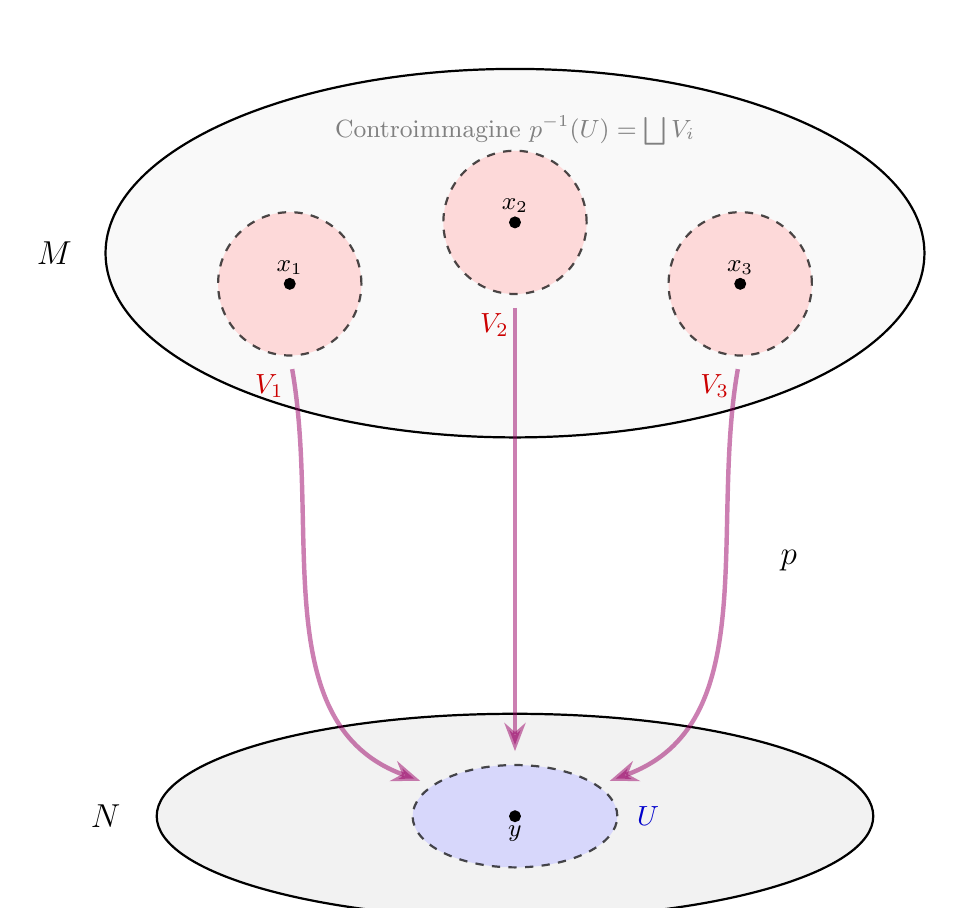
\begin{tikzpicture}[>=Stealth, scale=1.3]
		
		% --- SPAZIO BASE X (in basso) ---
		% Il manifold base
		\draw[fill=gray!10, thick] (0,-3) ellipse (3.5cm and 1cm);
		\node[font=\large] at (-4, -3) {$N$};
		
		% Il punto y
		\coordinate (y) at (0,-3);
		
		% L'intorno U banalizzante
		% Usiamo un'ellisse tratteggiata per l'aperto
		\draw[dashed, fill=blue!20, opacity=0.7, thick] (y) ellipse (1cm and 0.5cm);
		\node[blue!80!black, font=\bfseries] at (1.3, -3) {$U$};
		\filldraw (y) circle (1.5pt) node[below, font=\small] {$y$};
		
		
		% --- SPAZIO TOTALE \tilde{X} (in alto) ---
		% Disegniamo una grande ellisse che rappresenta una porzione di \tilde{X}
		\draw[fill=gray!5, thick] (0, 2.5) ellipse (4cm and 1.8cm);
		\node[font=\large] at (-4.5, 2.5) {$M$};
		\node[font=\small, gray] at (0, 3.7) {Controimmagine $p^{-1}(U) = \bigsqcup V_i$};
		
		% --- LE "PALLE" V_i (Controimmagini) ---
		% Definiamo i centri delle tre palle
		\coordinate (yt1) at (-2.2, 2.2);
		\coordinate (yt2) at (0, 2.8);
		\coordinate (yt3) at (2.2, 2.2);
		
		% Palla V_1
		\draw[dashed, fill=red!20, opacity=0.7, thick] (yt1) circle (0.7cm);
		\filldraw (yt1) circle (1.5pt) node[above, font=\small] {$x_1$};
		\node[red!80!black, font=\bfseries] at ($(yt1)+(-0.2,-1)$) {$V_1$};
		
		% Palla V_2 (quella centrale)
		\draw[dashed, fill=red!20, opacity=0.7, thick] (yt2) circle (0.7cm);
		\filldraw (yt2) circle (1.5pt) node[above, font=\small] {$x_2$};
		\node[red!80!black, font=\bfseries] at ($(yt2)+(-0.2,-1)$) {$V_2$};
		
		% Palla V_3
		\draw[dashed, fill=red!20, opacity=0.7, thick] (yt3) circle (0.7cm);
		\filldraw (yt3) circle (1.5pt) node[above, font=\small] {$x_3$};
		\node[red!80!black, font=\bfseries] at ($(yt3)+(-0.25,-1)$) {$V_3$};
		
		
		% --- MAPPE DI PROIEZIONE p ---
		% Frecce grosse che mostrano che l'intero insieme V_i va in U
		
		% Freccia da V1 a U
		\draw[->, ultra thick, opacity=0.5, red!60!blue, shorten >= 5pt, shorten <= 5pt] 
		($(yt1)+(0,-0.7)$) to[out=-80, in=160] ($(y)+(-0.8, 0.3)$);
		
		% Freccia da V2 a U (centrale)
		\draw[->, ultra thick, opacity=0.5, red!60!blue, shorten >= 5pt, shorten <= 5pt] 
		($(yt2)+(0,-0.7)$) -- ($(y)+(0, 0.5)$);
		
		% Freccia da V3 a U
		\draw[->, ultra thick, opacity=0.5, red!60!blue, shorten >= 5pt, shorten <= 5pt] 
		($(yt3)+(0,-0.7)$) to[out=-100, in=20] ($(y)+(0.8, 0.3)$);
		
		% Etichetta della mappa
		\node[font=\large, right] at (2.5, -0.5) {$p$};
		
	\end{tikzpicture}
	\caption{Sketch grafico della \protect\circled{3} richiesta dalla definizione di mappa di rivestimento. In questo caso, se la mappa $p$ soddisfa la \protect\circled{1}, \protect\circled{2} allora sarebbe una mappa a $3$ fogli.}
\end{figure}

Vediamo qualche esempio di mappa di rivestimento: l'esempio più semplice è quello rappresentato dalla funzione $w = f(z) = z^n$ con $f: S^1 \to S^1$ che mappa il cerchio unitario
nel cerchio unitario. E' chiaro che preso $w \in S^1$, allora esistono $n$ soluzioni all'equazione $z^n = w$, dunque diremo che è una mappa a $n$ fogli.
\begin{figure}[htbp]
    \centering
    \begin{tikzpicture}[>=Stealth, scale=1.3]

        % --- SPAZIO BASE S^1 (sotto) ---
        \begin{scope}[shift={(0,-3)}]
            % Intera circonferenza base (grigio chiaro per indicare la varietà totale)
            \draw[thick, gray!50] (0,0) ellipse (2.5 and 1);
            \node[font=\large] at (-3.2, 0) {$S^1$};
            
            % Intorno banalizzante U (arco blu) - es. da -30° a 30°
            \draw[ultra thick, blue!80] ({2.5*cos(-30)}, {1*sin(-30)}) arc (-30:30:2.5 and 1);
            
            % Punto y sulla base (usiamo il punto 1)
            \filldraw (2.5, 0) circle (1.5pt) node[right, font=\small, black] {$1$};
            \node[blue!80!black, font=\bfseries] at (2.8, 0.5) {$U$};
        \end{scope}

        % --- SPAZIO TOTALE S^1 (sopra) ---
        \begin{scope}[shift={(0,2)}]
            % Intera circonferenza di rivestimento
            \draw[thick, gray!50] (0,0) ellipse (2.5 and 1);
            \node[font=\large] at (-3.2, 0) {$S^1$};
            
            % Preimmagine V1 (attorno a 0°) - da -10° a 10°
            % Essendo z^3, l'arco sopra è un terzo di quello sotto
            \draw[ultra thick, red!80] ({2.5*cos(-10)}, {1*sin(-10)}) arc (-10:10:2.5 and 1);
            \filldraw (2.5, 0) circle (1.5pt) node[right, font=\small, black] {$1$};
            \node[red!80!black, font=\bfseries] at (2.8, 0.4) {$V_1$};

            % Preimmagine V2 (attorno a 120°) - da 110° a 130°
            \draw[ultra thick, red!80] ({2.5*cos(110)}, {1*sin(110)}) arc (110:130:2.5 and 1);
            \filldraw ({2.5*cos(120)}, {1*sin(120)}) circle (1.5pt) node[above, font=\small, black] {$e^{i 2\pi/3}$};
            \node[red!80!black, font=\bfseries] at ({2.9*cos(120)}, {1.4*sin(120)-0.7}) {$V_2$};

            % Preimmagine V3 (attorno a 240°) - da 230° a 250°
            \draw[ultra thick, red!80] ({2.5*cos(230)}, {1*sin(230)}) arc (230:250:2.5 and 1);
            \filldraw ({2.5*cos(240)}, {1*sin(240)}) circle (1.5pt) node[below left, font=\small, black] {$e^{i 4\pi/3}$};
            \node[red!80!black, font=\bfseries] at ({2.9*cos(240)}, {1.4*sin(240)-0.15}) {$V_3$};
        \end{scope}

        % --- MAPPA DI PROIEZIONE p(z) = z^3 ---
        % Frecce che mostrano come i tre punti mappano tutti in 1
        \draw[->, thick, dashed, opacity=0.6, red!60!blue] (2.4, 1.8) -- (2.4, -2.8);
        
        \draw[->, thick, dashed, opacity=0.6, red!60!blue] 
            ({2.5*cos(120)}, {2+1*sin(120)-0.2}) to[out=-40, in=120] (2.4, -2.8);
            
        \draw[->, thick, dashed, opacity=0.6, red!60!blue] 
            ({2.5*cos(240)+0.2}, {2+1*sin(240)-0.2}) to[out=-10, in=160] (2.4, -2.8);

        % Etichetta della funzione
        \node[font=\large, fill=white, inner sep=2pt] at (4, -0.5) {$p(z) = z^3$};

    \end{tikzpicture}
    \caption{Rappresentazione della mappa di rivestimento $p: S^1 \to S^1$ con $p(z)=z^3$. Un intorno $U$ di $S^1$ ha come controimmagine tre aperti disgiunti $V_1, V_2, V_3$, mappati tutti in $U$.}
\end{figure}

Un altro possibile esempio di mappa di rivestimento è quello di rappresentato dalla funzione $f(x) = e^{i 2 \pi x}$ con $f: \mathbb{R} \to S^1$: in questo caso siamo davanti ad una mappa di rivestimento (perché le controimmagini sono un infinito numerabile) ad infiniti fogli.

\begin{figure}[htbp]
    \centering
    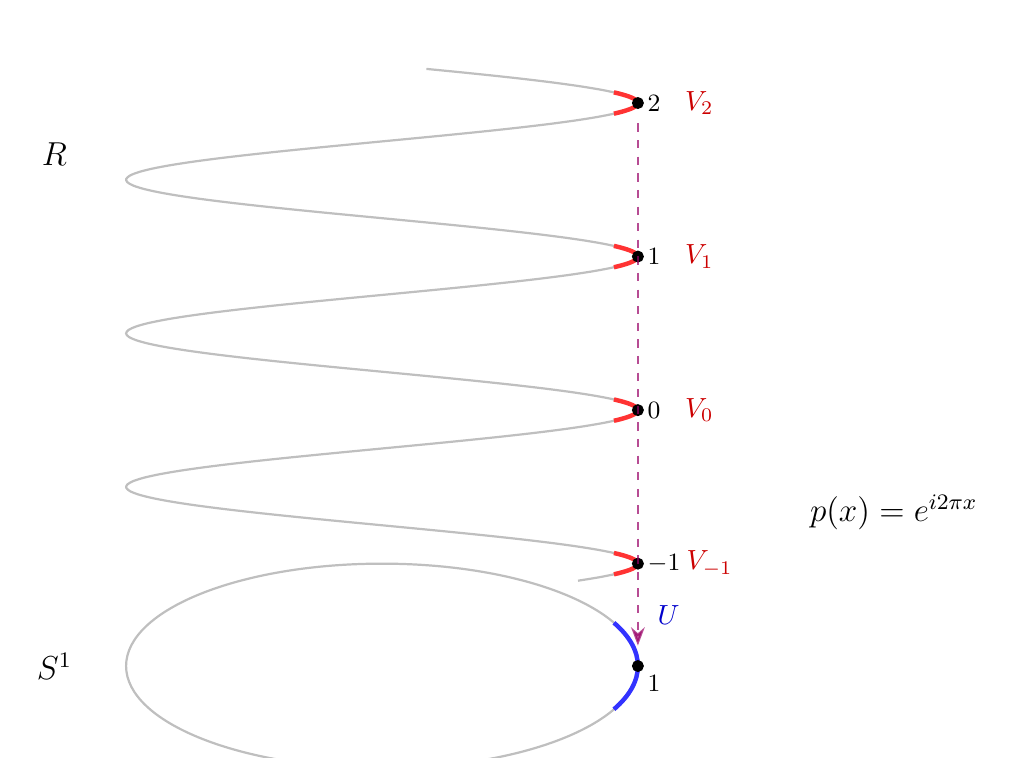
\begin{tikzpicture}[>=Stealth, scale=1.3]

        % --- SPAZIO BASE S^1 (sotto) ---
        \begin{scope}[shift={(0,0)}]
            % Circonferenza base
            \draw[thick, gray!50] (0,0) ellipse (2.5 and 1);
            \node[font=\large] at (-3.2, 0) {$S^1$};
            
            % Intorno banalizzante U (da -25° a 25°)
            \draw[ultra thick, blue!80] ({2.5*cos(-25)}, {1*sin(-25)}) arc (-25:25:2.5 and 1);
            
            % Punto 1 sulla base
            \filldraw (2.5, 0) circle (1.5pt) node[below right, font=\small, black] {$1$};
            \node[blue!80!black, font=\bfseries] at (2.8, 0.5) {$U$};
        \end{scope}

        % --- SPAZIO TOTALE R (L'elica, sopra) ---
        \begin{scope}[shift={(0,1)}]
            \node[font=\large] at (-3.2, 4) {$\mathbb{R}$};
            
            % Disegniamo l'elica parametrica. 
            % Un giro completo (360 gradi) avanza di 1.5 sull'asse verticale.
            \draw[thick, gray!50, domain=-400:800, samples=150, smooth, variable=\t] 
                plot ({2.5*cos(\t)}, {1.5 + \t/240});
            
            % --- CONTROIMMAGINI V_k (gli "scalini" sull'elica) ---
            
            % k = -1 (attorno a -360 gradi)
            \draw[ultra thick, red!80, domain=-385:-335, samples=20, smooth, variable=\t] 
                plot ({2.5*cos(\t)}, {1.5 + \t/240});
            \filldraw ({2.5*cos(-360)}, {1.5 + -360/240}) circle (1.5pt) node[right, font=\small, black] {$-1$};
            \node[red!80!black, font=\bfseries] at (3.2, {1.5 + -360/240}) {$V_{-1}$};

            % k = 0 (attorno a 0 gradi)
            \draw[ultra thick, red!80, domain=-25:25, samples=20, smooth, variable=\t] 
                plot ({2.5*cos(\t)}, {1.5 + \t/240});
            \filldraw ({2.5*cos(0)}, {1.5 + 0/240}) circle (1.5pt) node[right, font=\small, black] {$0$};
            \node[red!80!black, font=\bfseries] at (3.1, {1.5 + 0/240}) {$V_0$};

            % k = 1 (attorno a 360 gradi)
            \draw[ultra thick, red!80, domain=335:385, samples=20, smooth, variable=\t] 
                plot ({2.5*cos(\t)}, {1.5 + \t/240});
            \filldraw ({2.5*cos(360)}, {1.5 + 360/240}) circle (1.5pt) node[right, font=\small, black] {$1$};
            \node[red!80!black, font=\bfseries] at (3.1, {1.5 + 360/240}) {$V_1$};
            
            % k = 2 (attorno a 720 gradi)
            \draw[ultra thick, red!80, domain=695:745, samples=20, smooth, variable=\t] 
                plot ({2.5*cos(\t)}, {1.5 + \t/240});
            \filldraw ({2.5*cos(720)}, {1.5 + 720/240}) circle (1.5pt) node[right, font=\small, black] {$2$};
            \node[red!80!black, font=\bfseries] at (3.1, {1.5 + 720/240}) {$V_2$};
        \end{scope}

        % --- MAPPA DI PROIEZIONE p ---
        % Una freccia tratteggiata che scende verticalmente unendo tutti i numeri interi e finendo nell'1
        \draw[->, thick, dashed, opacity=0.7, red!60!blue] (2.5, {1 + 1.5 + 720/240 - 0.2}) -- (2.5, 0.2);

        % Etichetta della funzione
        \node[font=\large, fill=white, inner sep=2pt] at (5, 1.5) {$p(x) = e^{i 2\pi x}$};

    \end{tikzpicture}
    \caption{La mappa di rivestimento $p: \mathbb{R} \to S^1$. La retta reale $\mathbb{R}$ si avvolge a spirale infinite volte attorno alla circonferenza. L'intorno aperto $U$ ha come controimmagine infiniti aperti disgiunti $V_k$.}
\end{figure}

\section{Classificazione dei gruppi e sottogruppi}

Torniamo adesso ai gruppi: osserviamo che gli assiomi di gruppo non garantiscono la proprietà commutativo, quindi, se $(G_1, \circ)$ è un gruppo, allpresi $g_1, g_2 \in G$ generalmente si ha che
\begin{equation}
	g_1 \circ g_2 \neq g_2 \circ g_1.
\end{equation}

Ci sono, tuttavia, dei gruppi per cui vale anche la proprietà commutativa: un esempio molto importante che vedremo è $\text{SO}(2)$.
\begin{definition}
	Sia $(G, \circ)$ un gruppo, diremo che $G$ è un gruppo abeliano se
	\begin{equation}
		\forall g_1, g_2 \in G, g_1 \circ g_2 = g_2 \circ g_1
	\end{equation}
\end{definition}

\begin{definition}[commutatore]
	Sia $(G, \circ)$ un gruppo, definiamo il commutatore di $g_1, g_2 \in G$ come
	\begin{equation}
		\{ g_1, g_2 \} = g_1 \circ g_2 \circ (g_1)^{-1} \circ (g_2)^{-1}.
	\end{equation}
\end{definition}

Vale la seguente proposizione

\begin{prop}
	Sia $(G, \circ)$ un gruppo, se
	\begin{equation}
		\forall g_1, g_2 \in G, \{ g_1, g_2 \} = e \iff G \text{ è abeliano},
	\end{equation}
\end{prop}
\begin{exercise}
	Mostrare questa proposizione per esercizio.
\end{exercise}

\begin{proof}[Svolgimento] \hspace{1cm} \\
	$\boxed{\Leftarrow}$: chiaramente, se vale la proprietà commutativa allora
	\begin{equation}
		\{ g_1, g_2 \} = g_1 \circ g_2 \circ (g_1)^{-1} \circ (g_2)^{-1} = g_2 \circ g_1 \circ (g_1)^{-1} \circ (g_2)^{-1} = g_2 \circ (g_2)^{-1} = e.
	\end{equation}
	$\boxed{\Rightarrow}$: se $\forall g_1, g_2 \in G$ si ha che $\{ g_1, g_2 \}$ allora è chiaro che
	\begin{align}
		&g_1 \, \circ \, g_2 \, \circ \, (g_1)^{-1} \, \circ \, (g_2)^{-1} = e \implies g_1 \, \circ \, g_2 \, \circ \, (g_1)^{-1} \, \circ \, (g_2)^{-1} \, \circ \, (g_2) = e \, \circ \, g_2 \implies \nonumber \\
		&\implies g_1 \circ g_2 \circ (g_1)^{-1} \circ g_1 = g_2 \circ g_1 \implies g_1 \circ g_2 = g_2 \circ g_1,
	\end{align}
	e la tesi segue dall'arbitrarietà di $g_1$ e $g_2$.
\end{proof}

Ovviamente possiamo parlare anche di \emph{finitezza} di un gruppo,

\begin{definition}[gruppo finito]
	Sia $(G, \circ)$ un gruppo, diremo che $G$ è un gruppo finito se possiede un numero finito di elementi, altrimenti è infinito.
\end{definition}

Un esempio di gruppo finito è, chiaramente, il gruppo rappresentato dalle soluzioni all'equazione $z^3 = 1$, mentre un gruppo infinito può essere $(\mathbb{Z}, +)$. In base al ``tipo" di infinito degli elementi, possiamo parlare di \emph{gruppi continui},

\begin{definition}[gruppi continui]
	Sia $(G, \circ)$ un gruppo, diremo che $G$ è un gruppo continuo se $\{ g_i \} \in G$ è un insieme con cardinalità del continuo di elementi.
\end{definition}

Siccome i gruppi sono spazi topologici, si può dare anche la nozione di compattezza di un gruppo continuo,
\begin{definition}[gruppo compatto]
	Sia $(G, \circ)$ un gruppo, diremo che è compatto $\{ g_i \} \in G$ è un intervallo limitato di elementi.
\end{definition}

\begin{exercise}
	Mostrare che esiste un unico gruppo di ordine 2
\end{exercise}
\begin{proof}
	Per farlo, consideriamo la tabella moltiplicativa
	\begin{table}[H]
		\centering
		\begin{tabular}{c | c c}
			\, & e & a \\
			\hline
			e & e & a \\
			a & a & e
		\end{tabular}
	\end{table}
	A meno di isomorfismi, la struttura moltiplicativa del gruppo è identica.
\end{proof}

\begin{exercise}
	Mostrare che esiste un unico gruppo di ordine 3
\end{exercise}
\begin{proof}
	Per farlo, consideriamo la tabella moltiplicativa
	\begin{table}[H]
		\centering
		\begin{tabular}{c | c c c}
			\, & e & a & b \\
			\hline
			e  & e & a & b \\
			a  & a & b & e \\
			b  & b & e & a \\
		\end{tabular}
	\end{table}
	Vediamo che questa è l'unica tabella commutativa permessa, poiché altrimenti avremmo un assurdo
\end{proof}

\subsection{Sottogruppi e coset}

Come abbiamo fatto negli spazi vettoriali, in cui dato uno $\mathbb{K}-$spazio vettoriale $V$ ci siamo soffermati nello studio dei sottospazi, ovvero dei sottoinsiemi di $V$ che
possiedono la struttura di spazio vettoriale con la legge di composizione interna ed esterna di $V$, vogliamo adesso studiare degli insiemi di $(G, \circ)$ gruppo che sono ancora dei
gruppi rispetto alla $\circ$. Diremo che questi insiemi sono dei \emph{sottogruppi}

\begin{definition}[sottogruppi]
	Sia $(G, \circ)$ un gruppo, diremo che $H \subseteq G$ è un sottogruppo di $G$ se
	\begin{enumerate}[label=\protect\circled{\arabic*}]
		\item $\{ h_i \} \in G$;
		\item $\forall i, j, h_i \circ h_j \in H$ e $e \in H$.
	\end{enumerate}
\end{definition}
\begin{remark}
	Questa definizione è perfettamente equivalente a dire che $(H, \circ)$ è un gruppo (in maniera simile a quando dicevamo che $W \subseteq V$ spazio vettoriale è sottospazio di $V \iff \forall \alpha, \beta \in \mathbb{K}, \forall \underline{v}, \underline{w} \in W, \alpha \cdot_ V \underline{v} +_V \beta \cdot_V \underline{w} \in W$.)
\end{remark}
\begin{remark}
	Chiaramente $\{ e \} = H$ e $H = G$ sono i sottogruppi banali.
\end{remark}

\textbf{Notazione:} quando scriveremo $H$, salvo espresso diversamente, intenderemo sempre un sottogruppo non banale.

Una tipologia di sottogruppo molto importante sono quelli \emph{invarianti}

\begin{definition}[sottogruppo invariante]
	Sia $(G, \circ)$ un gruppo, diremo che $H \subseteq G$ è un sottogruppo invariante se
	\begin{equation}
		\forall g_i \in G, \forall h_k \in H, g_i h_k g_i^{-1} \in H,
	\end{equation}
	oppure in forma più simbolica
	\begin{equation}
		\forall g_i \in G, g_i H g_i^{-1} \in H
	\end{equation}
\end{definition}

In base alla presenza o meno di sottogruppi invarianti, è possibile andare a categorizzare ulteriormente i gruppi

\begin{definition}[gruppo semplice e semi-semplice]
	Sia $(G, \circ)$ un gruppo, diremo che
	\begin{enumerate}[label=\protect\circled{\arabic*}]
		\item diremo che $G$ è un gruppo \textbf{semplice} se è un gruppo \underline{senza} un sottogruppo invariante;
		\item diremo che $G$ è un gruppo \textbf{semi-semplice} se è un gruppo \underline{senza} un sottospazio invariante abeliano.
	\end{enumerate}
\end{definition}
\begin{remark}
	Chiaramente si ha che
	\begin{figure}[H]
		\centering
		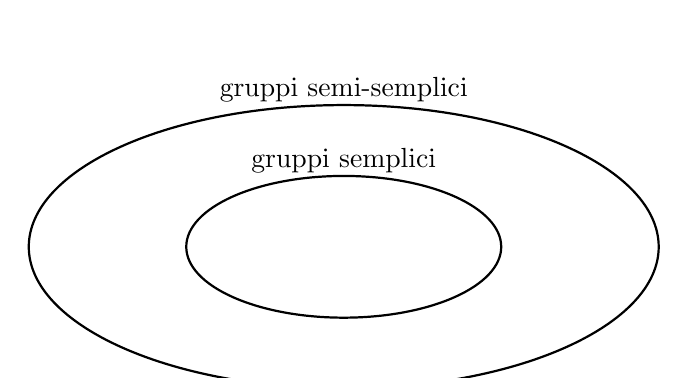
\begin{tikzpicture}
			\draw[fill=white, thick] (0, 2.5) ellipse (4cm and 1.8cm);
			\node[font=\normalsize] at (0, 4.5) {gruppi semi-semplici};
			\draw[fill=white, thick] (0, 2.5) ellipse (2cm and 0.9 cm);
			\node[font=\normalsize] at (0, 3.6) {gruppi semplici};
		\end{tikzpicture}
		\caption{Relazione insiemistica fra gruppi semplici e semi-semplici}
	\end{figure}
\end{remark}

Un altro oggetto molto importante, che possiamo definire a partire da un sottogruppo è il concetto di \emph{coset}
\begin{definition}[coset]
	Sia $(G, \circ)$ un gruppo,sia $g_i \in G$ e sia $H \subset G$ un sottogruppo, diremo che il coset sinistro di $H$ con \emph{rappresentante} $g_i$ è l'insieme degli elementi dati da
	\begin{equation}
		g_i \, \circ \, H. 
	\end{equation}
	L'insieme di tutti i coset è indicato con $G \, \backslash \, H$.
\end{definition}
\begin{remark}
	In pratica, stiamo vedendo gli elementi della forma $g_1 \circ h_1, g_1 \circ h_2, \ldots$ come il medesimo elemento, ovvero il coset di $H$ con rappresentante $g_i$: si potrebbe dare una definizione alternativa
	tramite relazione d'equivalenza dicendo che
	$$
		g_i \sim_H g_j \iff g_i^{-1} g_j \in H \iff g_j \in g_i H 
	$$
\end{remark}

\begin{remark}
	Si potrebbe definire anche il coset destro (noi sopra abbiamo fatto quello sinistro), come l'insieme degli elementi, fissato $g_i \in G$, della forma
	\begin{equation}
		H \, \circ \, g_i.
	\end{equation}
\end{remark}

Solitamente il coset non ha una struttura di gruppo rispetto a $\circ$, tuttavia si può mostrare che
\begin{prop} \label{prop:sott_inv_coset_grupp}
	Sia $(G, \circ)$ un gruppo e sia $H \subseteq G$ un sottogruppo invariante, allora $\equivcls{G}{H}$ è un gruppo rispetto a $\circ$
\end{prop} 
\begin{proof}
	Si ha infatti che presi $g_1 \circ H$ e $g_2 \circ H$ allora, essendo $H$ un sottogruppo invariante
	\begin{equation}
		g_1 \circ H \circ g_2 \circ H \stackrel{e = g_2 \circ g_2^{-1}}{=} g_1 \circ g_2 \circ \underbrace{g_2^{-1} H \circ g_2}_{\in H} H = g_1 \circ g_2 \circ H.
	\end{equation}
\end{proof}

\section{Omomorfismi}

Vogliamo analizzare, adesso, una classe di mappe fra gruppi molto importanti, che rispettano la struttura algebrica del gruppo. Prima di definire esplicitamente cosa siano, vediamo una situazione generale:
consideriamo due gruppi, che indichiamo con $(G_1, \circ_1), (G_2, \circ_2)$, e consideriamo una mappa $f: G_1 \to G_2$; in generale, si vede che, presi $a, b \in G_1$ abbiamo che
\begin{equation} \label{eq:strutt_alg}
	f(a \circ_1 b) \neq f(a) \circ_2 f(b).
\end{equation}
Questa proprietà di rispettare le operazioni fra i gruppi è ciò che si intende col rispettare la struttura algebrica del gruppo. Le mappe che rispettano la (\ref{eq:strutt_alg}) sono ciò che noi chiamiamo \textbf{omomorfismi}, di cui riportiamo la definizione formale qua sotto

\begin{definition}[omomorfismo]
	Siano $(G_1, \circ_1)$ e $(G_2, \circ_2)$ due gruppi (non necessariamente distinti), diremo che $f: G_1 \to G_2$ è un omomorfismo se
	\begin{equation}
		\forall a, b \in G_1, f(a \circ_1 b) = f(a) \circ_2 f(b).
	\end{equation}
\end{definition}

E' facile mostrare che
\begin{exercise}
	Siano $(G_1, \circ_1)$ e $(G_2, \circ_2)$ due gruppi e sia $f: G_1 \to G_2$ un omomorfismo, allora
	\begin{enumerate}[label=\protect\circled{\arabic*}]
		\item se $e_1$ è l'elemento neutro di $G_1$ e $e_2$ è l'elemento neutro di $G_2$, allora
		\begin{equation}
			f(e_1) = e_2,
		\end{equation}
		\item se $a \in G_1$, allora
		$$
			f(a^{-1}) = (f(a))^{-1}.
		$$
	\end{enumerate}
\end{exercise}
\begin{proof}
	Mostriamo la \circled{1}: è facile vedere, usando il fatto che $e_1 = e_1 \circ e_1$, che
	\begin{align}
		f(e_1) &= f(e_1 \, \circ_1 \, e_1) = f(e_1) \, \circ_2 \, f(e_1) \implies f(e_1) \, \circ_2 \, (f(e_1))^{-1} = f(e_1) \, \circ_2 \, f(e_1) \, \circ_2 \,(f(e_1))^{-1} \nonumber \\
		&\implies e_2 = f(e_1),
	\end{align}
	dove abbiamo usato il fatto che $G_2$ è comunque un gruppo, dunque ad ogni elemento esiste un suo inverso.
	Mostriamo la \circled{2}: 
	\begin{align}
		e_2 &= f(e_1) = f(a^{-1} \circ_1 a) = f(a^{-1}) \circ_2 f(a) \implies e_2 \circ_2 (f(a))^{-1} = f(a^{-1}) \circ_2 f(a) \circ_2 (f(a))^{-1} = \nonumber \\
			&= f(a^{-1}) \circ_2 e_2 = f(a^{-1}) \implies (f(a))^{-1} = f(a^{-1}).
	\end{align}
\end{proof}
Possiamo introdurre, similmente a come avevamo fatto per le applicazioni lineari fra spazi vettoriali, il kernel di un omomorfismo

\begin{definition}[kernel di un omomorfismo]
	Siano $(G_1, \circ_1)$ e $(G_2, \circ_2)$ due gruppi e sia $f: G_1 \to G_2$ un omorfismo fra i due. Allora definiamo kernel di $f$ come
	\begin{equation}
		\text{Ker}(f) = \{ g_1 \in G_1 : f(g_1) = e_2 \}.
	\end{equation}
\end{definition}
\begin{prop}
	$\text{Ker}(f)$ è un sottospazio invariante.
\end{prop}
\begin{proof}
\begin{align}
	&g^{-1} \circ_1 \text{Ker}(f) \circ_1 g \mapsto f(g^{-1}) \circ_2 f(\text{Ker}(f)) \circ_2 f(g) = (f(g))^{-1} \circ_2 e_2 \circ_2 f(g) = e_2 \implies \nonumber \\
	&\implies g^{-1} \circ (\text{Ker}(f)) \circ g \in \text{Ker}(f). 
\end{align}
\end{proof}
\begin{cor} \label{cor:g_ker_grupp}
	$\equivcls{G}{\, \text{Ker}(f)}$ è un gruppo rispetto a $\circ_G$.
\end{cor}
\begin{proof}
	E' sufficiente usare la \ref{prop:sott_inv_coset_grupp}.
\end{proof}

Tramite il kernel è possibile mostrare il seguente teorema

\begin{theorem}[Fondamentale degli omomorfismi]
    Siano $(G_1, \circ_1)$ e $(G_2, \circ_2)$ due gruppi e sia $f: G_1 \to G_2$ un omomorfismo surgettivo. Allora
    \begin{equation}
        G_1 / \text{Ker}(f) \cong \text{Im}(f)
    \end{equation}
\end{theorem}

% Per fare questa dimostrazione è necessario il seguente lemma:
% \begin{lemma} \label{lemma:eq_coset_ker}
% 	Sia $K$ il kernel di un omomorfismo $f: G_1 \to G_2$ con $(G_1, \circ_1)$ e $(G_2, \circ_2)$ due gruppi, allora $\forall a \in G_1$
% 	\begin{equation}
% 		aK = Ka.
% 	\end{equation}
% \end{lemma}
% \begin{proof}
% 	La dimostrazione verte nel far vedere che $aK \subseteq Ka$ e $Ka \subseteq aK$. Partiamo con la prima \\
% 	$\boxed{\subseteq}:$ sia $a \, \circ_1 \, k \in aK$, con $k \in K$, allora si ha che
% 	\begin{equation}
% 		f(a \, \circ_1 \, k \, \circ_1 \, a^{-1}) = f(a) \, \circ_2 \, f(k) \, \circ_2 \, f(a^{-1}) = f(a) \circ_2 (f(a))^{-1} = e_2,
% 	\end{equation}
% 	dunque $a \, \circ_1 k \, \circ_1 a^{-1} \in \text{Ker}(f),$ dunque $\exists k' \in K$ tale che
% 	\begin{equation}
% 		a \, \circ_1 k \, \circ_1 a^{-1} = k' \implies a \, \circ_1 k \, \circ_1 a^{-1} \, \circ_1 \, a = k' \, \circ_1 \, a,
% 	\end{equation}
% 	dunque $aK \subseteq Ka$. \\
% 	$\boxed{\supseteq}:$ sia $k \, \circ \, a \in Ka, k \in K$, allora si ha che
% 	\begin{equation}
% 		f(a^{-1} \, \circ_1 \, k \, \circ_1 \, a) = f(a^{-1}) \, \circ_2 \, f(k) \, \circ_2 \, f(a) = e_2,
% 	\end{equation}
% 	dunque $a^{-1} \, \circ_1 k \, \circ_1 \, a \in \text{Ker}(f)$, dunque $\exists k' \in K$ tale che
% 	\begin{equation}
% 		a^{-1} \, \circ_1 k \, \circ_1 \, a = k' \implies a \, \circ_1 a^{-1} \, \circ_1 k \, \circ_1 \, a = a \, \circ_1 \, k' \implies k \, \circ_1 \, a = a \, \circ_1 \, k',
% 	\end{equation}
% 	quindi $Ka \subseteq aK$.
% \end{proof}
\begin{proof}
    Sia $K = \text{Ker}(f)$. Si osserva che, se $a, a' \in G_1$ tali che $f(a) = f(a') = a^\star \in \text{Im}(f)$ allora
    \begin{equation}
        a^{-1} \, \circ_1 a' \stackrel{f}{\mapsto} f(a^{-1}) \, \circ_2 \, f(a') = (f(a))^{-1} \, \circ_2 \, f(a') = (a^\star)^{-1} \, \circ_2 \, a^\star = e_{2}, 
    \end{equation}
    dunque abbiamo che
    \begin{equation}
        a^{-1} \, \circ_1 \, a' \in K.
    \end{equation}
    Tuttavia si ha, a questo punto, che
    \begin{equation}
        a \, \circ_1 \, K = a \, \circ_1 \, (a^{-1} \, \circ_1 \, a') K = (a \, \circ_1 \, a^{-1}) \, \circ_1 \, a' K = a' \, \circ_1 \, K,
	\end{equation}
    dove abbiamo usato il fatto che se $k \in K \implies k \, \circ_1 \, K = K$, siccome $K$ ha la struttura di sottogruppo e $a^{-1} \, \circ_1 \, a' \in K$. 
    Dunque la mappa $\bar{f}$ che associa ad ogni coset di $K$ il valore di $f$ applicato all'elemento rappresentante del coset (ovvero $\bar{f}(aK) = f(a)$) è ben definita ed iniettiva. 
    
    Inoltre, la mappa è surgettiva su $\text{Im}(f)$: per definizione, $\forall b \in \text{Im}(f), \exists a \in G_1 : f(a) = b$, dunque $\exists aK \in G_1 / K : \bar{f}(aK) = b$.

    Infine, la mappa conserva l'operazione di gruppo: è sufficiente osservare che per la \ref{cor:g_ker_grupp} si ha che
    \begin{align}
        \bar{f}(aK \circ_1 bK) = \bar{f}(a \circ bK) = f(a \circ b) = f(a) \circ_2 f(b) = \bar{f}(aK) \circ_2 \bar{f}(bK).
    \end{align}
    Essendo biunivoca e un omomorfismo, $\bar{f}$ è un isomorfismo.
\end{proof}

Una particolare rilevante di isomorfismi è quello di \emph{automorfismo}, ovvero un isomorfismo da un gruppo in sé stesso. E' chiaro che l'insieme degli automorfismi sia un gruppo
rispetto all'operazione di composizione: sia $(G, \cdot)$ un gruppo e siano $g_1, g_2 : G \to G$ automorfismi, allora è chiaro che la funzione $g_1 \cdot g_2 : G \to G$ è ben definita e preso $a, b \in G$ abbiamo che
\begin{equation}
	(g_1 \circ g_2)(a \cdot b) = g_1(g_2(a \cdot b)) = g_1(g_2(a) \cdot g_2(b)) = g_1(g_2(a)) \cdot g_1(g_2(b)) = (g_1 \circ g_2)(a) \cdot (g_1 \circ g_2)(b),
\end{equation}
altrettanto chiaro è il fatto che, in generale, abbiamo
\begin{equation}
	g_1 \circ g_2 \neq g_2 \circ g_1.
\end{equation}
\begin{definition}[automorfismo e insieme degli automorfismi]
	Sia $(G, \circ)$ un gruppo e sia $f: G \to G$ un isomorfismo, diremo allora che $f$ è un automorfismo e indicheremo l'insieme degli automorfismi con $\text{Aut}(G)$. 
\end{definition}

Un automorfismo particolarmente rilevante è il concetto di \emph{automorfismo indotto}: sia $(G, \circ)$ un gruppo e sia $g \in G$ fissato, allora l'applicazione

\begin{equation}
	g \in G \mapsto h \, \circ \, g \,  \circ \, h^{-1} \in G,
\end{equation}

in quanto è suriettivo (preso $g \in G,$ allora abbiamo sicuramente che $h^{-1} \, \circ \, g \, \circ \, h$ è controimmagine di $g$) ed è iniettivo (siccome se $f(g_1) = f(g_2) \implies 
h \, \circ \, g_1 \, \circ \, h^{-1} = h \, \circ \, g_2 \, \circ \, h^{-1} \implies g_1 \, \circ \, h^{-1} = g_2 \, \circ \, h^{-1} \implies g_1 = g_2$) e il fatto che sia un omomorfismo deriva dal fatto che

\begin{equation}
	g_1 \, \circ \, g_2 \mapsto h \, \circ \, g_1 \, \circ g_2 \, \circ \, h^{-1} = h \, \circ \, g_1 \, \circ \, h^{-1} \, \circ \, h \, \circ \, g_2 \, \circ \, h^{-1} = f(g_1) \, \circ \, f(g_2). 
\end{equation}

	\chapter{Gruppi e algebre di Lie}

Molti dei gruppi che compaiono in Fisica hanno una struttura continua: si pensi a $\text{SO}(3)$, $\text{SO}(4)$, $\text{SU}(2)$ e $\text{SU}(4)$, i cui
elementi dipendono da un set continuo di variabili che variano su un intervallo. Quello che caratterizza i gruppi di Lie, tuttavia, è il fatto di possedere una funzione
differenziabile che lega 
\begin{definition}[gruppo di Lie]
    Sia $(G, \circ)$ un gruppo continuo, i cui elementi sono indicati da un insieme di parametri continui $\{ \alpha \} = \{ \alpha_1, \ldots, \alpha_n \}$ ovvero
    \begin{equation}
        A \in G, A = A(\alpha) = A(\alpha_1, \ldots, \alpha_n)
    \end{equation}
    per cui risulti che
    \begin{equation}
        e = A(\mathbf{0}) = A(0, \ldots, 0),
    \end{equation}
    con le seguenti proprietà:
    \begin{enumerate}[label=\protect\circled{\arabic*}]
        \item \textbf{chiusura}:
        \begin{equation}
            A(\alpha) \circ A(\beta) = A(\gamma),
        \end{equation}
        dove $\gamma = f(\alpha, \beta)$ con $f$ funzione differenziabile tale che
        \begin{equation}
            f(0, \alpha) = \alpha, f(\beta, 0) = \beta;
        \end{equation}
        \item \textbf{inversa}:
        \begin{equation}
            (A(\alpha))^{-1} = A(\alpha'),
        \end{equation}
        dove $\alpha' = g(\alpha)$ è una funzione differenziabile in $\alpha$;
        \item \textbf{associatività}:
        \begin{equation}
            A(\alpha) \, \circ \, (A(\beta) \, \circ \, A(\gamma)) = (A(\alpha) \, \circ \, A(\beta)) \, \circ \, A(\gamma),
        \end{equation}
        che implica che
        \begin{equation}
            f(\alpha, f(\beta, \gamma)) = f(f(\alpha, \beta), \gamma).
        \end{equation}
    \end{enumerate}
    Allora diremo che $G$ è un gruppo di Lie.
\end{definition}
Diamo al momento una piccola anticipazione del concetto di rappresentazione: essa è, sostanzialmente, un omomorfismo fra un gruppo e un gruppo di matrici, per cui $T \mapsto M(T)$ e $T_1 \circ T_2 \mapsto M(T_1) M(T_2)$ (dove si sottointende
il prodotto di matrici)

Uno dei risultati sicuramente più importanti sui gruppi di Lie si ha introducendo le misura di Haar, che definiamo come
\begin{definition}[misura di Haar]
    Sia $(G, \circ)$ un gruppo, diremo che $dg$ è una misura di Haar se
    \begin{enumerate}[label=\protect\circled{\arabic*}]
        \item \textbf{normalizzazione:} 
        \begin{equation}
            \int_G dg = 1,
        \end{equation}
        \item $\forall b \in \mathbb{R}$,
        \begin{equation}
            \int_G dg bf(g) = b \int_G dg f(g),
        \end{equation}
        \item se $\forall g \in G, f(g) \geq 0$ allora
        \begin{equation}
            \int_G dg f(g) \geq 0,
        \end{equation}
        \item \textbf{linearità:} se $a, b \in \mathbb{R}$
        \begin{equation}
            \int_G dg (af_1(g) + b f_2(g)) = a \int_G dg f_1(g) + b \int_G dg f_2(g).
        \end{equation}
        \item \textbf{invariante a destra e sinistra:} se $a \in G$, allora
        \begin{align}
            \int_G dg f(a \circ g)  = \int_G f(g) = \int_G dg f(g \circ a),
        \end{align}
        e
        \begin{align}
            \int_G dg^{-1} f(g) = \int_G f(g).
        \end{align}
    \end{enumerate}
\end{definition}

Vale che
\begin{theorem}
    Se $(G, \circ)$ è un gruppo di Lie \textbf{compatto}, allora $\exists$ una misura invariante di Haar.
\end{theorem}
Non daremo una dimostrazione di questo fatto, tuttavia ci concentreremo nel fornire alcuni esempi.
\begin{example} \hspace{1cm} \\
    \begin{enumerate}[label=\protect\circled{\arabic*}]
        \item Si consideri il gruppo $(\mathbb{R}_{> 0}, \circ = \cdot)$: tale insieme è un gruppo siccome presi $x, y \in \mathbb{R}_{> 0}$ si ha che
        \begin{equation}
            x \circ y = x \cdot y \in \mathbb{R}_{> 0},
        \end{equation}
        inoltre si ha che soddisfa la richiesta di esistenza dell'elemento neutro (ovvero $1 \in \mathbb{R}_{> 0}$), di associatività (la moltiplicazione sui reali è chiaramente associativa)
        e di esistenza di elemento inverso per ogni elemento del gruppo (preso $x \in \mathbb{R}_{> 0}$, allora $\frac{1}{x} \in \mathbb{R}_{> 0}$ e $x \circ \frac{1}{x} = 1$). Si osservi che questo gruppo \textbf{non} è compatto, tuttavia è
        possibile trovare comunque una misura di Haar. Si osserva infatti che se $dg = dx$ non si ha una misura di Haar, siccome
        \begin{equation}
            \int_{\mathbb{R}_{> 0}} dg f(a \circ g) \stackrel{t = ax}{=} \frac{1}{a} \int_{\mathbb{R}_{> 0}} f(t) dt \neq \int_{\mathbb{R}_{> 0}} f(g)dg,  
        \end{equation}
        ma, in maniera ancora più drammatica si ha che,
        \begin{equation}
            \int_{\mathbb{R}_{> 0}} dx = +\infty,
        \end{equation}
        tuttavia, se $dg = \frac{dx}{x}$ allora
        \begin{equation}
            \int_{\mathbb{R}_{> 0}} dg f(a \circ g) \stackrel{t = ax}{=} \int_{\mathbb{R}_{> 0}} f(t) \frac{dt}{t}.
        \end{equation}
        \item Si consideri $\text{SO}(2)$: tale gruppo è compatto siccome i parametri dipendono da $\theta \in [0, 2 \pi]$, dunque il gruppo è compatto. Si ha che se $R = R(\theta) \in \text{SO}(2)$, allora $R(\theta_1) \circ R(\theta_2) = R(\theta_1 + \theta_2)$ e in questo caso si ha che $dg = \frac{1}{2 \pi} d\theta$, da cui è possibile mostrare che
        \begin{equation}
            \int_{\text{SO}(2)} dg f(g) = \int_{0}^{2 \pi} \frac{d\theta}{2 \pi} = 1.
        \end{equation}
        \item Si consideri il gruppo $\text{SU}(2)$. Una sua possibile parametrizzazione è data dalla matrice:
            \begin{equation}
                U = \begin{pmatrix}
                    a & b \\
                    -b^{\ast} & a^{\ast}
                \end{pmatrix}
            \end{equation}
            con la condizione che $U^\dagger U = \mathbf{1}$ e $\det{U} = 1$. Si osserva che se poniamo:
            \begin{equation}
                \begin{cases}
                    a = x_1 + i y_1 \\
                    b = x_2 + i y_2
                \end{cases}
            \end{equation}
            allora dalla condizione sul determinante segue immediatamente che:
            \begin{equation}
                x_1^2 + y_1^2 + x_2^2 + y_2^2 = 1,
            \end{equation}
            dunque si ha l'identificazione (a meno di un diffeomorfismo) $\text{SU}(2) \sim S^3$. 

            Un modo per costruire la misura di Haar è osservare che possiamo parametrizzare questo gruppo con $3$ angoli. Una prima parametrizzazione utile per studiare il gruppo in termini di fasi e moduli è:
            \begin{equation}
                U = \begin{pmatrix}
                    e^{i \frac{\alpha}{2}} \cos{\theta} & e^{i \frac{\beta}{2}} \sin{\theta} \\
                    -e^{-i \frac{\beta}{2}} \sin{\theta} & e^{-i \frac{\alpha}{2}} \cos{\theta}
                \end{pmatrix},
            \end{equation}
            dove i parametri variano negli intervalli $\theta \in \left[0, \frac{\pi}{2}\right]$, mentre $\alpha, \beta \in [0, 4\pi)$ per poter coprire in modo completo la varietà.

            Tuttavia, per ricavare esplicitamente l'elemento di misura, risulta più comodo sfruttare direttamente la geometria di $S^3$. Se fossimo in $S^2$, avremmo che:
            \begin{equation}
                x_1^2 + x_2^2 + x_3^2 = 1 \implies d\Omega(S^2) = \sin{\theta} \, d\theta \, d\phi,
            \end{equation}
            dove $d\Omega(S^2)$ è l'elemento infinitesimo di superficie. Nel caso di $S^3$ la costruzione è analoga ma richiede un passo in più. Dalla condizione iniziale abbiamo che:
            \begin{equation}
                x_1^2 + y_1^2 + x_2^2 + y_2^2 = 1 \implies x_2^2 + y_1^2 + y_2^2 = 1 - x_1^2.
            \end{equation}
            Essendo la somma di quadrati non negativa, si deve avere $1 - x_1^2 \geq 0$, da cui $x_1^2 \leq 1$. Possiamo quindi porre:
            \begin{equation}
                x_1 = \cos{\theta} \quad \text{con } \theta \in [0, \pi].
            \end{equation}
            dove l'intervallo è limitato a $\pi$ per garantire l'iniettività ed evitare di ricoprire la sfera due volte. Ne consegue che:
            \begin{equation}
                x_2^2 + y_1^2 + y_2^2 = 1 - \cos^2{\theta} = \sin^2{\theta},
            \end{equation}
            e quindi la terna $(x_2, y_1, y_2)$ è costretta a ``vivere" su una superficie sferica bidimensionale $S^2$ di raggio $\sin{\theta}$. Parametrizzando questa terna con le coordinate sferiche consuete, introduciamo due angoli $\alpha \in [0, \pi]$ e $\beta \in [0, 2\pi)$:
            \begin{equation}
                \begin{cases}
                    x_2 = \sin{\theta} \sin{\alpha} \cos{\beta} \\
                    y_1 = \sin{\theta} \sin{\alpha} \sin{\beta} \\
                    y_2 = \sin{\theta} \cos{\alpha}
                \end{cases}
            \end{equation}
            L'elemento di volume (ovvero la misura di Haar) su $S^3$ si costruisce combinando la variazione lungo $\theta$ con l'elemento d'area della sfera di raggio $\sin{\theta}$:
            \begin{equation}
                d\Omega(S^3) = \sin^2{\theta} \, d\theta \, d\Omega(S^2).
            \end{equation}
            Sostituendo l'espressione per $d\Omega(S^2) = \sin{\alpha} \, d\alpha \, d\beta$, si ottiene infine:
            \begin{equation}
                dg \propto \sin^2{\theta} \sin{\alpha} \, d\theta \, d\alpha \, d\beta.
            \end{equation}
            dove il proporzionale è necessario perché manca il termine di normalizzazione, che si può facilmente ricavare calcolando il valore dell'integrale su $S^3$
            \begin{equation}
                \int_0^{\pi} \int_{0}^\pi \int_{0}^{2 \pi} \sin^2{\theta} \sin{\alpha} \, d\theta \, d\alpha \, d\beta = 2 \pi \int_{0}^\pi \sin^{2}(\theta) d \theta \int_{0}^\pi \sin{\alpha} d\alpha, 
            \end{equation}
            e ricordando che
            \begin{equation}
                \int_0^{\pi} \sin^2{\theta} d\theta = \int_0^{\pi} \frac{1 - \cos(2\theta)}{2} d\theta = \int_{0}^\pi d\theta = \frac{\pi}{2},
            \end{equation}
            e che
            \begin{equation}
                \int_0^\pi \sin{\alpha} d\alpha = 2,
            \end{equation}
            si conclude che
            \begin{equation}
                \int_0^{\pi} \int_{0}^\pi \int_{0}^{2 \pi} \sin^2{\theta} \sin{\alpha} \, d\theta \, d\alpha \, d\beta = 2 \pi^2,
            \end{equation}
            da cui segue che per rispettare la $\circled{1}$ si deve avere che
            \begin{equation}
                dg = \frac{1}{2 \pi^2} \sin^2{\theta} \sin{\alpha} \, d\theta \, d\alpha \, d\beta.
            \end{equation}
            Si può facilmente verificare che questa misura è effettivamente una misura di Haar.
            \begin{figure}[H]
                \centering
                \includegraphics[width=\textwidth]{immagini/SU(2)_explanation.png}
                \caption{Spiegazione delle coordinate scelte per la parametrizzazione di $\text{SU}(2)$}
            \end{figure}
            \item L'ultimo esempio che consideriamo è quello del gruppo delle matrici triangolari $2 \times 2$, ovvero le matrici della forma
            \begin{equation}
                T = \begin{pmatrix}
                    a & b \\
                    0 & c
                \end{pmatrix},
            \end{equation}
            con la condizione che $ac \neq 0 \, (\iff a \neq 0 \wedge c \neq 0 \text{ per il principio di annullamento del prodotto})$. Tramite la parametrizzazione delle matrici con $a, b, c$ è immediato far vedere che l'insieme delle matrici triangolari $2 \times 2$ è un gruppo: prese due matrici triangolari, infatti, si ha che
            \begin{equation}
                T_1 T_2 = \begin{pmatrix}
                    a_1 & b_1 \\
                    0 & c_1
                \end{pmatrix} \begin{pmatrix}
                    a_2 & b_2 \\
                    0 & c_2
                \end{pmatrix} = \begin{pmatrix}
                    a_1 a_2 & a_1 b_2 + b_1 c_2 \\
                    0 & c_1 c_2 
                \end{pmatrix},
            \end{equation}
            che è ancora una matrice triangolare e $a_1 a_2 c_1 c_2 \neq 0$ (siccome sarebbe equivalente a chiedere che $a_1 \neq 0 \wedge a_2 \neq 0 \wedge c_1 \neq 0 \wedge c_2 \neq 0$ sempre per il principio di annullamento del prodotto, ma ciò è garantito dal fatto che sappiamo che vale contemporaneamente il fatto che $a_1 c_1 \neq 0$ e $a_2 c_2 \neq 0$).
            Osserviamo che se vogliamo imporre che la misura di Haar sia invariante ``a sinistra", ovvero che
            \begin{equation}
                \int_G dg f(g) = \int_G dg f(a \circ g), 
            \end{equation}
            con $a \in G$ fissato, si deve avere che col cambiamento di variabile $t = a \circ g$ la misura $dg(t) = dt$: si ha allora che se
            \begin{equation}
                T_x = \begin{pmatrix}
                    x & y \\
                    0 & z
                \end{pmatrix},
            \end{equation}
            è l'elemento di gruppo integrato e
            \begin{equation}
                T = \begin{pmatrix}
                    a & b \\
                    0 & c
                \end{pmatrix},
            \end{equation}
            è l'elemento $a$ fissato, allora
            \begin{equation}
                T T_x = \begin{pmatrix}
                    ax & ay + bz \\
                    0  & cz
                \end{pmatrix} = \begin{pmatrix}
                    x' & y' \\
                    0 & z'
                \end{pmatrix},
            \end{equation}
            osserviamo che allora con il cambiamento di variabile $t = a \circ g$, allora
            \begin{equation}
                \begin{cases}
                    x' = ax \\
                    y' = ay + bz \\
                    z' = cz
                \end{cases},
            \end{equation}
            e calcolando la matrice jacobiana si ha che lo jacobiano risulta essere
            \begin{equation}
                \det{\begin{bmatrix}
                    a & 0 & 0 \\
                    0 & b & c \\
                    0 & 0 & c
                \end{bmatrix}} = a^2 c,
            \end{equation}
            dunque
            \begin{equation}
                dx' dy' dz' = a^2 c dx dy dz = \left( \frac{x'}{x} \right)^2 \frac{z'}{z} dx dy dz \implies \frac{dx' dy' dz'}{(x')^2 z'} = \frac{dx dy dz}{x^2 z},
            \end{equation}
            risulta quindi che 
            
            \begin{equation} \label{eq:mis_triang_destra}
                dg = \frac{dx dy dz}{x^2 z}
            \end{equation}
            
            è la misura cercata. Ripetendo il conto, tuttavia, si scopre che la misura invariante \emph{a destra} è diversa da questa trovata:
            il motivo sta chiaramente nel fatto che questo gruppo \textbf{non} è compatto, dunque non è garantita l'esistenza di una misura di Haar invariante a destra e sinistra.
            \begin{exercise}
                Trovare la misura invariante a destra di questo gruppo
            \end{exercise}
            \begin{proof}[Svolgimento]
                E' sufficiente osservare che, fissando una matrice $T$ della forma
                \begin{equation}
                    T = \begin{pmatrix}
                        a & b \\
                        0 & c
                    \end{pmatrix},
                \end{equation}
                e una matrice $T_x$ (che sarà quella ``integrata") si ha che
                \begin{equation}
                    T_x T = \begin{pmatrix}
                        x & y \\
                        0 & z
                    \end{pmatrix} \begin{pmatrix}
                        a & b \\
                        0 & c
                    \end{pmatrix} = \begin{pmatrix}
                        ax & bx + cy \\
                        0  & cz
                    \end{pmatrix},
                \end{equation} 
                dunque lo jacobiano della trasformazione risulta essere pari a
                \begin{equation}
                    \det{\begin{pmatrix} a & 0 & 0 \\ b & c & 0 \\ 0 & 0 & c \end{pmatrix}} = ac^2,
                \end{equation}
                da cui si ottiene che
                \begin{equation}
                    dx' dy' dz' = ac^2 dxdydz = \left( \frac{x'}{x} \right) \left(\frac{z'}{z} \right)^2 dx dy dz \implies \frac{dx' dy' dz'}{x' (z')^2} = \frac{dx dy dz}{x z^2}.
                \end{equation}
                Concludiamo che la misura di questo gruppo invariante a sinistra sia $dg = \frac{dx dy dz}{x z^2}$ che è distinta dalla misura vista in \ref{eq:mis_triang_destra}.
            \end{proof}
    \end{enumerate}
\end{example}
\section{Algebra di Lie}
Vogliamo adesso descrivere il comportamento del gruppo in un \emph{intorno} dell'identità di un gruppo di Lie: per fare questo si introduce il concetto di \emph{generatore infinitesimo del gruppo $G$}.

\begin{definition}
    Sia $G$ un gruppo di Lie per cui $g(\{ \alpha \}) \in G$ e si consideri una rappresentazione $g \mapsto M(g) = M({\alpha})$, definiamo il \emph{generatore infinitesimo del gruppo $G$} come
    \begin{equation}
        T^i = -i \frac{\partial M(\alpha)}{\partial \alpha_i} \bigg|_{\{ \alpha \} = 0}.
    \end{equation}
\end{definition}

Questi generatori entrano in gioco considerando l'espansione in serie di Taylor di una matrice $M(\{ \alpha \})$, ovvero si ha che
\begin{equation}
    M(\{ \alpha \}) = \mathbf{1} + i \alpha_i T^i + \ldots
\end{equation}


Si postula, nella nostra trattazione, che i $\{ T^i \}$ posseggano le seguenti proprietà:
\begin{enumerate}[label=\protect\circled{\arabic*}]
    \item formino uno spazio vettoriale, che chiameremo \emph{algebra del gruppo $G$}, quindi
    \begin{equation}
        \{ T^a \} \in \text{Alg}(G) \, (\text{oppure scriveremo } \mathfrak{g}),
    \end{equation}
    nel senso che
    \begin{equation}
        c_1 T^1 + c_2 T^2 + \ldots + c_n T^n \in \mathfrak{g},
    \end{equation}
    e ciò implica che anche lo $\mathbf{0} \in \mathfrak{g}$
    \item il set $\{ T^a \}$ è chiuso per commutazioni, ovvero
    \begin{equation} \label{eq:comm_inf}
        [T^a, T^b] \stackrel{\text{def.}}{\equiv} T^a T^b - T^b T^a \in \mathfrak{g}.
    \end{equation}
\end{enumerate}
Da queste è possibile provare, abbastanza facilmente, che siccome $\mathfrak{g}$ ha la struttura di spazio vettoriale, allora è possibile scegliere i generatori
in maniera tale che siano ortogonali rispetto alla traccia (conseguenza del teorema di Lagrange)
$$
    \text{Tr}(T^a T^b) = C \delta^{ab},
$$
dove la costante $C$ è detto indice di Dynkin e dipende dalla rappresentazione scelta (vedremo poi che, fissando un indice di Dynkin, allora gli altri indici delle altre rappresentazioni saranno fissati).
Prendendo una base opportuna di $\mathfrak{g}$, possiamo dire che la condizione espressa in (\ref{eq:comm_inf}) equivale a
\begin{equation}
    [T^a, T^b] = i f^{abc} T^c,
\end{equation}  
e segue chiaramente dal fatto che $[T^a, T^b] = -[T^b, T^a]$ che $f^{bac} = - f^{abc}$. Possiamo dire di più, in realtà, osservando che moltiplicando per $T^d$ da entrambi i lati
\begin{equation} \label{eq:ant_comm}
    [T^a, T^b] T^d = i f^{abc} T^c T^d \implies \text{Tr}([T^a, T^b] T^d)=\text{Tr}(i f^{abc} T^c T^d) = i f^{abc} \text{Tr}(T^c T^d) = i f^{abc} C \delta^{cd},
\end{equation}
da cui, prendendo $T^d = T^c$, si ottiene che
\begin{equation}
    iCf^{abc} = \text{Tr}([T^a, T^b] T^c) = \text{Tr}(T^a T^b T^c - T^b T^a T^c) \implies f^{abc} = - \frac{i}{C} (\text{Tr}(T^a T^b T^c) - \text{Tr}(T^b T^a T^c)), 
\end{equation}
e sfruttando la proprietà della traccia
\begin{equation}
    \text{Tr}(AB) = \text{Tr}(BA),
\end{equation}
si ottiene che
\begin{align}
    f^{abc} &= - \frac{i}{C} (\text{Tr}(T^a T^b T^c) - \text{Tr}(T^b T^a T^c)) = - \frac{i}{C} (\text{Tr}(T^b T^c T^a) - \text{Tr}(T^c T^b T^a)) = f^{bca} = \\
    &= - \frac{i}{C} (\text{Tr}(T^c T^a T^b) - \text{Tr}(T^a T^c T^b)) = f^{cab},
\end{align}
dove le espressioni di $f^{bca}$ e $f^{cab}$ sono ottenute ragionando come sopra in (\ref{eq:ant_comm}).
Una domanda che finora non abbiamo risposto sarebbe ``\emph{qual è il miglior modo per parametrizzare un gruppo?}" Nel caso di $\text{SO}(2)$, per esempio, abbiamo una grande libertà di scelta dovuto al fatto che l'angolo è definito a
meno di $2 k \pi$, tuttavia la scelta più saggia per i nostri scopi sarebbe la \emph{parametrizzazione esponenziale}, per cui risulta che
\begin{equation}
    R(\{ \alpha \}) = e^{i \alpha^a T^a},
\end{equation}
che può essere interpretato come un'iterazione di trasformazioni infinitesime successive, ottenendo così un elemento finito
\begin{equation}
    \lim_{k \to + \infty} \left( \mathbf{1} + i \frac{\alpha_a T^a}{k} \right)^k,
\end{equation}
che risulta consistente con la definizione data dei generatori. \\
La necessità della commutazione fra i generati entra in gioco quando si considera il commutatore ``usuale'' che abbiamo definito nei gruppi: se consideriamo degli elementi molto ``vicini'' all'identità, sappiamo che
\begin{align}
&g_1 \approx \mathbf{1} + i \alpha T - \frac{1}{2}(\alpha T)^2, \
&g_2 \approx \mathbf{1} + i \beta T - \frac{1}{2}(\beta T)^2,
\end{align}
da cui si ha che
\begin{align}
&g_1^{-1} \approx \mathbf{1} - i \alpha T - \frac{1}{2}(\alpha T)^2 \
&g_2^{-1} \approx \mathbf{1} - i \beta T - \frac{1}{2}(\beta T)^2,
\end{align}
da cui segue che
\begin{align}
    &g_1^{-1} \circ g_2^{-1} \circ g_1 \circ g_2 =  \\
    &= (\mathbf{1} - i \alpha T - (\alpha T)^2) \circ (\mathbf{1} - i \beta T - (\beta T)^2) \circ (\mathbf{1} + i \alpha T - (\alpha T)^2) \circ (\mathbf{1} + i \beta T - (\beta T)^2) \\
    &= (\mathbf{1} - i \beta T - (\beta T)^2 - i \alpha T + (\alpha T) (\beta T) + i (\alpha T) (\beta T)^2 - (\alpha T)^2 + i (\alpha T)^2 (\beta T) + (\alpha T)^2 (\beta T)^2) \circ \\
    &( \mathbf{1} + i \beta T - (\beta T)^2 + i \alpha T - (\alpha T)(\beta T) - i (\alpha T)(\beta T)^2 - (\alpha T)^2 - i (\alpha T)^2 (\beta T) + (\alpha T)^2 (\beta T)^2) = \\
    &= \mathbf{1} - (\alpha T)(\beta T) + (\beta T)(\alpha T) \\
    &= \mathbf{1} + \alpha^a \beta^b(T^b T^a - T^a T^b) = \mathbf{1} - \alpha^a \beta^b [T^a, T^b].
\end{align}
Per coerenza, si deve avere che questo elemento qua è ancora "sufficientemente" vicino all'identità, dunque è espandibile in serie, pertanto si deve avere che
\begin{align}
    &g_1^{-1} \circ g_2^{-1} \circ g_1 \circ g_2 = \mathbf{1} + i \gamma^c T^c + \ldots = \mathbf{1} - \alpha^a \beta^b [T^a, T^b] + \ldots = \mathbf{1} + i \gamma T^c \implies \\
    &\implies \alpha^a \beta^b [T^a, T^b] = i \gamma^c T^c.
\end{align}

\begin{figure}
    \centering
    \usetikzlibrary{positioning, calc}
    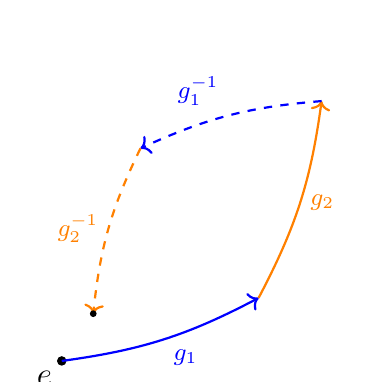
\begin{tikzpicture}
        % Punto di partenza (Identità)
        \coordinate (y) at (0,-3);
        \filldraw (y) circle (1.5pt) node[below left, font=\large] {$e$};
        
        % Cammino g1
        \draw[->, thick, blue] (y) to[bend right=10] 
            node[below right, font=\small] {$g_1$} ++(2.5, 0.8) coordinate (p1);
            
        % Cammino g2
        \draw[->, thick, orange] (p1) to[bend right=10] 
            node[right, font=\small] {$g_2$} ++(0.8, 2.5) coordinate (p2);
            
        % Cammino g1^{-1} (quasi opposto a g1, ma spostato sulla varietà)
        \draw[->, thick, blue, dashed] (p2) to[bend right=10] 
            node[above left, font=\small] {$g_1^{-1}$} ++(-2.3, -0.6) coordinate (p3);
            
        % Cammino g2^{-1} (non chiude il quadrato!)
        \draw[->, thick, orange, dashed] (p3) to[bend right=10] 
            node[left, font=\small] {$g_2^{-1}$} ++(-0.6, -2.1) coordinate (p4);

        % Punto finale
        \filldraw (p4) circle (1pt) node[above right, font=\small] {};

        % Il gap: il commutatore
        %\draw[->, thick, red] (y) -- (p4) 
        %    node[midway, left, font=\small, text=red] {$\mathbf{1} - [A, B]$};
    \end{tikzpicture}
    \caption{Rappresentazione del cammino infinitesimo $g_1^{-1} \circ g_2^{-1} \circ g_1 \circ g_2$. Nel caso di un gruppo non abeliano, l'iterazione delle trasformazioni dirette e inverse non riporta esattamente all'identità $e$. Il "gap" residuo è descritto dal commutatore dei generatori.}
\end{figure}

Si può mostrare che vale l'identità di Jacobi
\begin{prop}[identità di Jacobi]
    Sia $G$ un gruppo di Lie e sia $\mathfrak{g}$ con generatori $\{ T^a \} \in \mathfrak{g}$, allora
    \begin{align}
        [[T^a, T^b], T^c] + [[T^c, T^a], T^b] + [[T^b, T^c], T^a] = 0.
    \end{align}
\end{prop}
\begin{proof}
    \begin{align}
        &[[T^a, T^b], T^c] + [[T^c, T^a], T^b] + [[T^b, T^c], T^a] = \\
        &=[T^a T^b - T^b T^a, T^c] + [T^c T^a - T^a T^c, T^b] + [T^b T^c - T^c T^b, T^a] = \\
        &= T^a T^b T^c - T^b T^a T^c - T^c T^a T^b + T^c T^b T^a + \\
        &+ T^c T^a T^b - T^a T^c T^b - T^b T^c T^a + T^b T^a T^c + \\
        &+ T^b T^c T^a - T^c T^b T^a - T^a T^b T^c + T^a T^c T^b = 0.   
    \end{align}
\end{proof}

\begin{definition}[costanti di gruppo]
    Siano $\{ T^a \}$ i generatori infinitesimi di un gruppo di Lie $G$, allora si ha che
    \begin{align}
        [T^a, T^b] = i f^{abc} T^c,
    \end{align}
    dove $f^{abc}$ prendono il nome di \emph{costante del gruppo} e ne determinano l'algebra infinitesima.
\end{definition}

Una domanda che può sorgere è \emph{l'algebra di un gruppo determina univocamente il gruppo?} La risposta è \textbf{no}: infatti si ha che, in $\text{SO}(3)$ le costanti di gruppo sono le stesse di
$\text{SU}(2)$, quindi possiamo dire che il gruppo determina univocamente l'algebra associata, ma non il viceversa. 

Prendiamo come esempio sempre $SU(2)$: possiamo far vedere che i generatori di tale gruppo soddisfano la seguente relazione
\begin{align}
    [\frac{\sigma^a}{2}, \frac{\sigma^b}{2}] = i \epsilon^{abc} \frac{\sigma^c}{2},
\end{align}
(\emph{E' abbastanza semplice: si ha che
\begin{align}
    &\sigma^1 = \begin{pmatrix}
        0 & 1 \\
        1 & 0
    \end{pmatrix}, & &\sigma^2 = \begin{pmatrix}
        0 & -i \\
        i & 0
    \end{pmatrix}, & &\sigma^3 = \begin{pmatrix}
        1 & 0 \\
        0 & -1
    \end{pmatrix},
\end{align}
da cui si ha che
\begin{align}
    \left[ \frac{\sigma^1}{2}, \frac{\sigma^2}{2} \right] = \frac{1}{4} \left(\sigma^1 \sigma^2 - \sigma^2 \sigma^1 \right) = \frac{1}{4} \left(\begin{pmatrix}
        i & 0 \\
        0 & -i
    \end{pmatrix} - \begin{pmatrix}
        -i & 0 \\
        0 & i
    \end{pmatrix} \right) = \frac{1}{2} \begin{pmatrix}
        i & 0 \\
        0 & -i
    \end{pmatrix} = i \frac{\sigma^3}{2} = i \epsilon^{123} \frac{\sigma^3}{2}, 
\end{align}
e così per tutti gli altri.})
\begin{definition}[rappresentazione unitaria]
    Sia $G$ un gruppo e sia data una rappresentazione del gruppo, ovvero $g \in G \mapsto M(g)$ matrice, diremo che la rappresentazione è unitaria se
    \begin{align}
        M(g)M(g)^\dagger = \mathbf{1}.
    \end{align}
\end{definition}
Questo implica il fatto che i generatori siano hermitiani, infatti presa $U$ con
\begin{equation}
    U = e^{i \alpha^a T^a},
\end{equation}
allora
\begin{equation}
    U^\dag = e^{-i \alpha (T^\dagger)^\alpha} = U^{-1} = e^{i \alpha^a T^a} \implies (T^{\dagger})^a = T^a.
\end{equation}
Si può mostrare per esercizio che vale la seguente proprietà:
\begin{exercise}
    Sia $A = e^B$ allora
    \begin{align} \label{eq:tr_gen}
        \det{A} = e^{\text{Tr}(B)}.
    \end{align}
\end{exercise}
\begin{proof}
    Sappiamo, dal teorema di triangolarizzazione, che una matrice che ha tutte le radici del polinomio caratteristico nel campo di appartenenza è simile ad una matrice triangolare superiore, dunque
    \begin{align}
        \exists P \in \text{GL}(\mathbb{C}) : P^{-1} D P = B,
    \end{align}
    pertanto abbiamo che
    \begin{align}
        e^B = \sum_{n = 0}^{+\infty} \frac{B^n}{n!} = \sum_{k = 0}^{+\infty} \frac{(P^{-1} D P)^n}{n!} = P^{-1} \left( \sum_{k=0}^{+\infty} \frac{D^n}{n!} \right) P = P^{-1} e^D P,
    \end{align}
    da cui si ottiene che
    \begin{align}
        \det{e^B} = \det{P^{-1} e^D P} = \det{e^D} = e^{\lambda_1} e^{\lambda_2} \ldots e^{\lambda_n} = e^{\sum_{k = 1}^n \lambda_k} = e^{\text{Tr}(B)}.
    \end{align}
\end{proof}
\begin{remark}
    Nel caso reale, la dimostrazione è valida usando la forma canonica di Jordan, tuttavia è sufficiente osservare che, mettendoci in $\mathbb{C}$ e guardando ogni matrice reale come matrice complessa, la dimostrazione è sempre valida,
    oltre al fatto che il determinante è chiaramente reale siccome
    \begin{enumerate}
        \item il polinomio caratteristico è reale;
        \item le radici complesse, siccome i coefficienti sono tutti reali, devono presentarsi a coppie con il loro coniugato;
        \item la traccia è quindi reale;
        \item il determinante è, quindi, reale. 
    \end{enumerate}
\end{remark}

Abbiamo esplicitamente visto che i generatori di $\text{SU}(2)$ sono $3$, mentre $\text{SU}(3)$ ha le seguenti condizioni
\begin{enumerate}[label=\protect\circled{\arabic*}]
    \item $U U^\dagger = \mathbf{1} \implies$ i generatori devono essere hermitiani, quindi abbiamo che gli elementi sulla diagonale devono essere reali e gli elementi sono uno il coniugato dell'altro;
    \item $\det{U} = 1$, dunque si deve avere che i generatori hanno traccia nulla, usando l'esercizio mostrato sopra.      
\end{enumerate}
Si ottiene quindi che abbiamo
$$
    2 * 3^2 - 3 - 3(3-1) - 1 = 18 - 3 - 6 - 1 = 9 - 1 = 8,
$$
dove abbiamo tenuto di conto del fatto che, in totale, abbiamo inizialmente, con $n=3$, ben $2n^2$ numeri liberi (per ogni entrata abbiamo una parte reale e una parte immaginaria) e abbiamo usato il fatto che dobbiamo togliere $2 \frac{n^2 - n}{2}$ entrate sopra diagonale per
la condizione di hermitianeità (e il fattore $2$ tiene sempre di conto del fatto che abbiamo parte reale e immaginaria), mentre la condizione di determinante uguale a $1$ ci toglie un parametro libero. In generale si può mostrare che
\begin{exercise}
    Il numero di generatori di $\text{SU}(n)$ è pari a $n^2 - 1$.
\end{exercise}
\begin{proof}
    In linea teorica, i nostri generatori hanno, senza imporre alcun vincolo, ben $2n^2$ parametri liberi (il fattore $2$ tiene di conto sempre del fatto che abbiamo sia una parte reale che una parte complessa). Si ha, tuttavia, che il vincolo di $UU^\dagger = \mathbf{1}$ ci dice che i generatori
    devono essere hermitiani, quindi si ha che sulla diagonale abbiamo numeri reali (quindi vanno tolti $N$ parametri) e altrove abbiamo ben che gli elementi sopra diagonale vincolano quelli sotto e le entrate sopra diagonale sono $\frac{N(N-1)}{2}$ e per tenere conto di parte reale e complessa moltiplichiamo per $2$.
    Usando poi la (\ref{eq:tr_gen}) si ottiene che la traccia dei generatori dev'essere nulla, quindi si ha un solo vincolo (perché sappiamo già che gli elementi sulla diagonale sono reali). Si ha quindi che
    \begin{equation}
        2n^2 - 2 \, \frac{n(n-1)}{2} - n - 1 = n^2 - 1. 
    \end{equation}
\end{proof}
\begin{exercise}
    Il numero di generatori di $\text{SO}(n)$ è pari a
    \begin{align}
        \frac{n(n-1)}{2}
    \end{align}
\end{exercise}
\begin{proof}
    Si osserva che abbiamo $n$ numeri liberi e dalla condizione di trasposizione si ottiene che se
    \begin{align}
        A = e^{i \alpha^a T^a} \implies A^T A = e^{i \alpha^a (T^t)^a} e^{i \alpha^a T^{a}} = \mathbf{1} \implies e^{i \alpha^a (T^t)^a} = e^{-i \alpha^a T^a}, 
    \end{align}
    da cui si ha che
    \begin{align}
        T^t = -T,
    \end{align}
    ovvero i generatori sono matrici antisimmetriche. La condizione per cui il determinante dev'essere uno mi impone che la traccia dei generatori sia zero, tuttavia è già rispetta dal fatto che i generatori siano antisimmetrici: si conclude
    dunque che il numero di generatori di $\text{SO}(n)$ è pari a
    \begin{align}
        \frac{n(n-1)}{2}.
    \end{align}
\end{proof}
\begin{remark}
    Abbiamo usato il fatto che, presa $A_n$ successioni di matrici, la trasposizione è continua, ovvero
    \begin{align}
        (\lim_{n \to +\infty} A_n)^t = \lim_{n \to +\infty} A_n^t,
    \end{align}
    e distributiva rispetto alla somma di matrici, dunque, presa $B$ matrice e indicando con $S_n = \sum_{k=0}^n \frac{B^k}{k!}$, si ha
    \begin{align}
        (e^B)^t = \lim_{n \to +\infty} (S_n)^t = \lim_{n \to +\infty} (\sum_{k = 0}^{n} \frac{B^k}{k!})^t = \lim_{n \to +\infty} \sum_{k=0}^n \frac{(B^t)^k}{k!} = e^{B^t}. 
    \end{align}
\end{remark}
\begin{figure}[H]
    \centering
    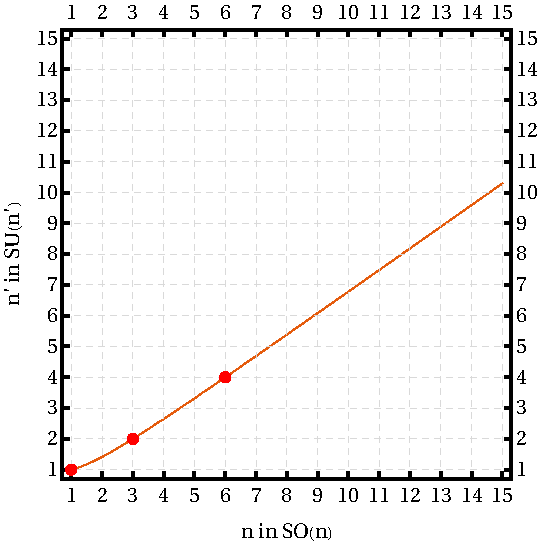
\includegraphics[width=\textwidth]{immagini/gen_so_su.pdf}
    \caption{Numero di generatori di $\text{SO}(n)$ e $\text{SU}(n')$. Si vede che per $n=1, n=3$ e $n=6$ abbiamo, rispettivamente, che i generatori di $SU(n')$ sono $n' = 1, n'=2$ e $n' = 4$: è possibile mostrare sono tutti valori per cui le algebre rispettive sono isomorfe.}
\end{figure}
\subsection{Sottoalgebre}

Come fatto per i gruppi, possiamo introdurre un concetto di sottoalgebra

\begin{definition}[sottoalgebra]
    Sia $G$ un gruppo di Lie e sia $\{ X^a\}$ un insieme di generatori dell'algebra $\mathfrak{g}$ di $G$. Sia $\mathfrak{h} \subseteq \mathfrak{g}$ con generatori
    \begin{align}
        Y^{{\dot{a}}} \in \mathfrak{h} \subseteq \mathfrak{g},
    \end{align}
    con
    \begin{align}
        [Y^{{\dot{a}}}, Y^{{\dot{b}}}] \in \mathfrak{h},
    \end{align}
    allora diremo che $\mathfrak{h}$ forma una sottoalgebra di $\mathfrak{g}$.
\end{definition}
Possiamo introdurre anche la nozione di \emph{sottoalgebra invariante}, che come vedremo va a generare dei sottogruppi invarianti

\begin{definition}[sottoalgebra invariante]
    Sia $G$ un gruppo di Lie e sia $\mathfrak{g}$ l'algebra di Lie di $G$ con generatori $\{ X^a \}$, sia $\mathfrak{h} \subseteq \mathfrak{g}$ una sottoalgebra con generatori $\{ Y^{\dot{a}} \}$, se
    \begin{align}
        \forall {\dot{a}}, b, [Y^{\dot{a}}, X^{b}] = c_d Y^d \in \mathfrak{h},
    \end{align}
    diremo che $\{Y^{\dot{a}} \}$ forma una sottoalgebra invariante o ideale di $\mathfrak{g}$. Se, inoltre,
    \begin{align}
        \forall {\dot{a}}, {\dot{b}}, [Y^{\dot{a}}, Y^{\dot{b}}] = 0,
    \end{align}
    diremo che $\mathfrak{h}$ forma una sottoalgebra invariante abeliana di $\mathfrak{g}$.
\end{definition}

\begin{prop}[le sottoalgebre generano sottogruppi invarianti]
    Sia $G$ un gruppo di Lie con $\mathfrak{g}$ algebra di Lie con generatori $\{ X^a \}$, sia $\mathfrak{h} \subseteq \mathfrak{g}$ un'algebra invariante con generatori $\{ Y^{\dot{a}} \}$, allora presi
    \begin{align}
        h = e^{i \alpha_{\dot{a}} Y^{\dot{a}}} \in H, g = e^{i \beta_b X^b} \in G, 
    \end{align} 
    si ha che
    \begin{align}
        g^{-1} h g \in H,
    \end{align}
    ovvero $H$ sottogruppo generato da $\mathfrak{h}$ è un sottospazio invariante di $G$.
\end{prop}
\begin{proof}
    Si osserva che
    \begin{align}
        g^{-1} h g = g^{-1} e^{i \alpha_{\dot{a}} Y^{\dot{a}}} g = e^{g^{-1} i \alpha_{\dot{a}} Y^{\dot{a}} g},
    \end{align}
    dove abbiamo usato il fatto che
    $$
        g^{-1} e^{A} g = g^{-1} \left( \sum_{k = 0}^{+\infty} \frac{A^k}{k!} \right) g = \sum_{k=0}^{+\infty} \frac{(g^{-1}Ag)^k}{k!} = e^{g^{-1} A g},
    $$
    in quanto $(g^{-1} A g)^n = (g^{-1} A g)^n = (g^{-1} A g)(g^{-1} A g) \ldots (g^{-1}Ag)(g^{-1} A g) = g^{-1} A^n g$.
    Si osserva che
    \begin{align}
        &(\mathbf{1} - i \alpha_{\dot{a}} Y^{\dot{a}} + \ldots) Y^{\dot{a}} (\mathbf{1} + i \alpha_{\dot{a}} Y^{\dot{a}} + \ldots) = \\
        &= Y^{\dot{a}} - \underbrace{i \beta_b[X^\beta, Y^{\dot{a}}]}_{{\in \mathfrak{h}}} + \frac{(-i)^2}{2!} \underbrace{[\beta \cdot X, [\beta \cdot X, Y]]}_{\in \mathfrak{h}} + \underbrace{\ldots}_{\in \mathfrak{h}} + \\
        &+\frac{(-i)^n}{n!}\underbrace{[\beta \cdot X, [\beta \cdot X, [\ldots, [\beta \cdot X, Y]]] \ldots]}_{\in \mathfrak{h}} + \underbrace{\ldots}_{\in \mathfrak{h}} = \\
        &= \gamma_{\dot{c}} Y^{\dot{c}} \in \mathfrak{h}.
    \end{align}
\end{proof}

\section{Gli strumenti per studiare i gruppi di Lee}

Lo scopo di questa sezione è quello di introdurre tutti gli strumenti con cui sarà possibile andare a studiare tutti i gruppi di interesse fisico.
Questi sono, principalmente, i seguenti:

\begin{enumerate}[label=\protect\circled{\arabic*}]
    \item mappe di rivestimento per studio delle proprietà locali e globali del gruppo;
    \item gruppi di omotopia superiori e non;
    \item gruppo di monodromia;
    \item teoria delle rappresentazioni. 
\end{enumerate}

\subsection{I gruppi di omotopia}

Abbiamo già visto le mappe di rivestimento, quindi partiamo a studiare i gruppi di omotopia: questo concetto si presta particolarmente bene negli spazi topologici connessi per archi:

\begin{definition}[spazio topologico]
    Sia $X$ un insieme e sia $\tau \subseteq \mathcal{P}(X)$, diremo che $\tau$ è una topologia di $X$ se
    \begin{enumerate}[label=\protect\circled{\arabic*}]
        \item $\emptyset, X \in \tau$;
        \item $\{ A_i \}_{i \in \mathbb{N}} \subseteq \tau \implies \bigcup\limits_{i=0}^{+\infty} A_i \in \tau$;
        \item se $k < +\infty, \{ A_i \}_{i \in \{ 1, \ldots, k\}} \subseteq \tau \implies \bigcap\limits_{i=0}^k A_i \in \tau$;
    \end{enumerate}
    e diremo che $(X,\tau)$ è uno spazio topologico.
\end{definition}

\begin{definition}[spazio topologico connesso per archi]
    Sia $(X, \tau)$ uno spazio topologico, diremo che è connesso per archi se $\forall x, y \in X, \, \exists \gamma : [0,1] \to X$ tale che $\gamma(0) = x, \gamma(1) = y$.
\end{definition}

Si osservi che prese due curve $\gamma_1: [0,1] \to X$ e $\gamma_2: [0,1] \to X$ con $\gamma_1(1)=\gamma_2(0)$ allora considerare la curva $\gamma = \gamma_1 \ast \gamma_2$ così definita
\begin{align}
    \gamma(t) = \begin{cases}
        \gamma_1(2t) & \text{se } 0 \leq t \leq \frac{1}{2}; \\
        \gamma_2(2(t - \frac{1}{2})) & \text{se } \frac{1}{2} \leq t \leq 1.
    \end{cases}
\end{align}
e quindi definire l'operazione di composizione di due curve $\ast$, che non gode, chiaramente, di proprietà associativa come vedremo sotto.

Prese due curve su uno spazio $X$, possiamo dare la nozione di equivalenza di una curva
\begin{definition}[curve equivalenti]
    Siano $\gamma_1 : [a,b] \to X$ e $\gamma_2 : [c,d] \to X$ con $\gamma_1(0) = \gamma_2(0)$ e $\gamma_1(1) = \gamma_2(1)$, diremo che $\gamma_1(t)$ è equivalente a $\gamma_2(\tau)$ se esiste $f(t) \in C^1([a, b], [c,d])$ tale che $\tau(a) = c, \tau(b) = d$ e $\tau = f(t)$ con $f'(t) > 0 \, \forall t \in [a,b]$ oppure, equivalentemente, si ha che
    \begin{align}
        \gamma_1(t) = \gamma_2(\tau(t)).
    \end{align}
\end{definition}

\begin{example}
    Come esempio di curve equivalenti possiamo considerare
    \begin{align}
        &\gamma_1(t) = (\cos{\left( \frac{\pi}{2} t \right)} ,\sin{\left( \frac{\pi}{2} t \right)}) & &\gamma_2(\tau) = (\cos{\left( \frac{\pi}{2} \sqrt{2} \tau \right), \sin{\left( \frac{\pi}{2} \sqrt{2} \tau \right)}})
    \end{align}
    con $t \in [0, 2]$ e $\tau \in [0, \sqrt{2}]$. Si vede che tramite la mappa $[0,1] \ni x \mapsto 2x$ l'intervallo $[0,1]$ viene mappato in quello $[0,2]$, mentre l'intervallo $[0,1]$ in $[0, \sqrt{2}]$ tramite la mappa $[0,1] \ni x \mapsto \sqrt{2} x$, quindi si ha che
    \begin{align}
        &\tilde{\gamma_1}(t) = \gamma(2t) = (\cos{\left( \frac{\pi}{\cancel{2}} \cancel{2}t \right)}, \sin{\left( \frac{\pi}{\cancel{2}} \cancel{2}t \right)}) & &\tilde{\gamma_2}(\tau) = \gamma_2(\sqrt{2} \tau) = (\cos{\left( \frac{\pi}{\cancel{2}} \cancel{\sqrt{2} \sqrt{2}} \tau \right)}, \sin{\left( \frac{\pi}{\cancel{2}} \cancel{\sqrt{2} \sqrt{2}}\tau \right)}),
    \end{align}
    dove $\tilde{\gamma_1}$ e  $\tilde{\gamma_2}$ hanno sostegno in $[0,1]$. Ne consegue, dunque, che tramite la mappa $f: [0, 2] \to [0, \sqrt{2}]$ dove $x \stackrel{f}{\mapsto} \frac{x}{\sqrt{2}}$, si ha che
    \begin{align}
        \gamma_1(t) = \gamma_2(f(t)),
    \end{align}
    e chiaramente $f(t)$ è $C^1([0, 2], [0, \sqrt{2}])$, dunque le due curve sono equivalenti
\end{example}

Possiamo dare, tuttavia, una nozione più forte dell'equivalenza fra curva, ovvero l'\emph{omotopia} fra esse

\begin{definition}[omotopia fra curve]
    Sia $(X, \tau)$ uno spazio topologico, diremo che due curve $\gamma_1(x):[0,1] \to X$ e $\gamma_2(x):[0,1] \to X$ sono omotope se esiste una funzione $F(x,t) : [0, 1] \times [0,1] \to X$ tale che
    \begin{enumerate}
        \item $F$ è continua;
        \item $F(x, 0) = \gamma_1(x)$;
        \item $F(x, 1) = \gamma_2(x)$.
    \end{enumerate}
\end{definition}
\begin{remark}
    In generale la nozione di omotopia è una nozione che si dà fra funzioni, non necessariamente alle curve e basta.
\end{remark}
\begin{remark}
    Due curve equivalenti sono omotopicamente equivalenti: infatti abbiamo che la funzione
    $$
        F(x, t) = (1-t)\gamma_1(x) + t\gamma_2(f(x)),
    $$
    è una funzione continua e
    \begin{align}
        &F(x, 0) = \gamma_1(x),& &F(x, 1) = \gamma_2(f(x)).
    \end{align}
\end{remark}

La nozione di omotopia è parecchio versatile quando consideriamo l'insieme di tutte le curve chiuse che iniziano e terminano in un punto $x_0 \in X$, che viene denotato $\Omega(x_0, X)$: è chiaro che, in un insieme connesso per archi,
presi due punti, tale insieme dipende anche dalle curve che vivono in un altro punto; siccome le curve chiuse attorno ad un punto possono essere costruite prendendo la curva continua $\gamma$ che connette il punto $x_0$ e $x_1$ e "sommarla" con una curva chiusa attorno a $x_1$ e
percorrere la curva $\gamma$ al contrario. Si potrebbe dimostrare che questo insieme non ha la struttura di gruppo rispetto all'operazione di composizione di curve: intuitivamente, le curve
\begin{align}
    &(\gamma \ast \lambda) \ast \mu, & &\gamma \ast (\lambda \ast \mu),
\end{align}
sono curve differenti, anche se fanno lo stesso percorso, perché hanno velocità diversa nel compiere i vari giri, però sono omotopicamente equivalenti.

\begin{figure}[H]
    \centering
    \begin{tikzpicture}[
        midarrow/.style={postaction={decorate, decoration={markings, mark=at position 0.5 with {\arrow{Latex}}}}},
        quarterarrow/.style={postaction={decorate, decoration={markings, mark=at position 0.25 with {\arrow{Latex}}}}},
        thirdquarterarrow/.style={postaction={decorate, decoration={markings, mark=at position 0.75 with {\arrow{Latex}}}}}
    ]
        % Ellisse di sfondo
        \draw[fill=gray!10, thick] (0,0) ellipse (5cm and 2cm);
        \node[font=\large] at (-1, -2.5) {$X$};
        
        % Curva originale da x_0 a x_1 con freccia nel mezzo
        \draw[midarrow, ultra thick, opacity=0.5, red!60!blue] 
        (-1,-0.7) to (1, 0.3);
        
        % Curva inversa da x_1 a x_0 con freccia nel mezzo
        % Ho impostato gli angoli di uscita (out) ed entrata (in) in modo che formi un "ciclo" visivo
        \draw[midarrow, ultra thick, opacity=0.5, red!60!blue] 
        (1, 0.4) to (-1, -0.6);
        
        % Nodi (etichette)
        \node[font=\large] at (-1, -1) {$x_0$};
        \node[font=\large] at (1.4, 0.5) {$x_1$};
        
        % Punti (cerchi neri)
        \draw[fill=black] (-1, -0.7) circle (0.1cm and 0.1cm);
        \draw[fill=black] (1, 0.3) circle (0.1cm and 0.1cm);
        
        % Cerchio finale
        \draw[quarterarrow, thirdquarterarrow, ultra thick, opacity=0.5, red!60!blue] (2, 0.3) circle (1cm);
    \end{tikzpicture}
    \caption{Costruzione di un cammino chiuso attorno ad $x_0$ usando una curva chiusa di $x_1$: questo ci fa ipotizzare che ci sia un qualche tipo di legame fra $\Omega(x_0, X)$ e $\Omega(x_1, X)$.}
\end{figure}

Per ottenere la struttura di gruppo, si potrebbe andare a quozientare l'insieme delle curve all'interno di $\Omega(x_0, X)$ con la relazione di omotopia (è facile verificare che si tratta di una relazione d'equivalenza) e, in tal caso, si riacquista anche la proprietà associativa se definiamo la composizione di curve
sulle classi di equivalenza omotopica delle curve.

\begin{definition}[gruppo fondamentale]
    Sia $(X, \tau)$ uno spazio topologico, diremo che il gruppo delle classi omotopiche di cammini orientabili in $\Omega(x_0, X)$ è il grupo fondamentale $\pi_1(x_0, X)$.  
\end{definition}

Il fatto più importante, tuttavia, che bisogna ricordare è il fatto che per un insieme connesso per archi, $\pi_1(x_0, X)$ non dipende dal punto $x_0 \in X$ preso\footnote{più precisamente, preso $(X, \tau)$ spazio topologico connesso per archi e $x_0, x_1 \in X$ con $x_0 \neq x_1$, allora esiste un isomorfismo
fra $\pi_1(x_0, X)$ e $\pi_1(x_1, X)$.}, dunque per spazi topologici connessi per archi $(X, \tau)$ indicheremo il gruppo fondamentale direttamente con

\begin{align}
    \pi_1(X).
\end{align}

\begin{remark}
    Se fossimo in un insieme non connesso per archi, potremmo comunque restringerci alle componenti connesse per archi e lì possiamo usare il fatto che il gruppo fondamentale non dipende dal punto `preciso' preso in quella componente connessa
\end{remark}

A questo punto si potrebbe generalizzare il ragionamento appena fatto per introdurre i gruppi di omotopia superiore:
\begin{definition}[Gruppi di omotopia superiore]
    L'$i$-esimo gruppo di omotopia $\pi_i(X, x_0)$ è l'insieme delle classi di omotopia delle mappe continue da $S^i$ a $X$ aventi come punto base $x_0$. Equivalentemente, possiamo definire il gruppo di omotopia superiore usando le classi di omotopia di mappe da $D^i$ a $X$ tali che il bordo venga mappato nel punto base, ovvero $f(S^{i-1}) = \{x_0\}$.
\end{definition}

Possiamo facilmente mostrare che su tale insieme è possibile andare a definire un `prodotto' di mappe che gli dà una struttura di gruppo. Prima di farlo, è necessario il seguente risultato:

\begin{theorem}
    Se $A, B$ sono spazi topologici (con rispettivamente $\tau_A$ e $\tau_B$ le due topologie) e se $f: A \to B$ è una mappa continua fra i due tale che $f = g \circ h$ con $h: A \to C$ e $g: C \to B$, e con $C$ spazio topologico contraibile, allora $f$ è omotopa alla mappa costante.
\end{theorem}
\begin{proof}[Idea della dimostrazione]
    Ci si può convincere di ciò poiché posso costruire l'omotopia fra la funzione $f$ e la mappa costante considerando:
    \begin{align}
        H(x, t) = g(C(h(x), t)),
    \end{align}
    dove $C(y, t)$ è l'omotopia garantita dal fatto che lo spazio $C$ è contraibile (ovvero deformabile con continuità ad un punto base).
\end{proof}

Prima di andare avanti, è comodo definire la mappa $\psi: S^i \to S^i_1 \vee S^i_2$: per capire cosa fa questa mappa, immaginate di avere una sfera e di separarla sull'equatore. In topologia, quozientare un insieme rispetto a dei punti vuol dire farli incollare: un esempio può essere un rettangolo che può diventare un cilindro se incollate una sola coppia di lati paralleli, come si può vedere in figura.

\begin{figure}[htbp]
    \centering
    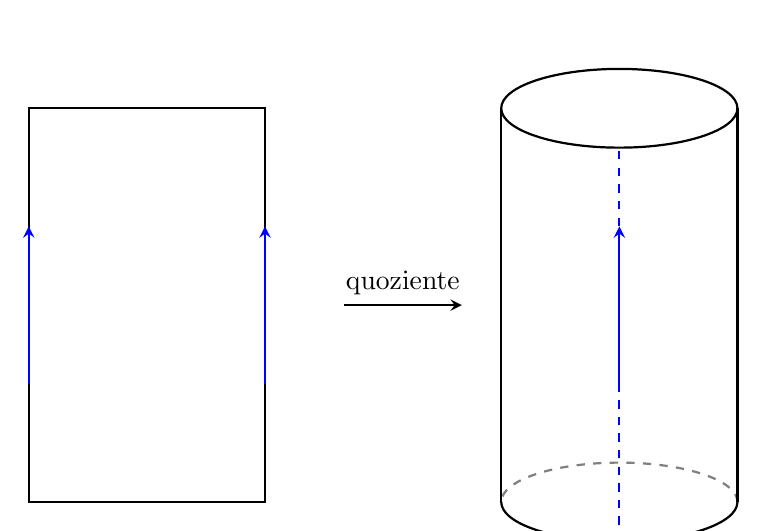
\begin{tikzpicture}[>=stealth, thick]
        % Definizione dello stile freccia
        \tikzset{arrow/.style={->, thick, blue}}
        
        % Rettangolo iniziale
        \draw[draw=black] (0,0) rectangle ++(3,5);
        
        % Frecce sui lati per indicare l'incollaggio (stesso verso)
        \draw[arrow] (0, 1.5) -- (0, 3.5);
        \draw[arrow] (3, 1.5) -- (3, 3.5);
        
        % Freccia che indica la trasformazione (quoziente)
        \draw[->] (4, 2.5) -- (5.5, 2.5) node[midway, above] {quoziente};
        
        % Cilindro risultante
        \begin{scope}[shift={(7.5, 0)}]
            % Base inferiore (ellisse a metà tratteggiata)
            \draw (-1.5,0) arc (180:360:1.5 and 0.5);
            \draw[dashed, opacity=0.5] (1.5,0) arc (0:180:1.5 and 0.5);
            
            % Base superiore (ellisse completa)
            \draw (0,5) ellipse (1.5 and 0.5);
            
            % Lati verticali esterni del cilindro
            \draw (-1.5,0) -- (-1.5,5);
            \draw (1.5,0) -- (1.5,5);
            
            % Linea di "cucitura" sul cilindro dove i lati si sono uniti
            \draw[dashed, blue] (0, -0.5) -- (0, 4.5);
            \draw[arrow] (0, 1.5) -- (0, 3.5);
        \end{scope}
    \end{tikzpicture}
    \caption{Quoziente di un rettangolo: incollare una coppia di lati paralleli per ottenere un cilindro.}
\end{figure}

Nel caso della sfera, quozientare tutto l'equatore in un punto equivale a chiudere la calotta sferica superiore e inferiore in un punto comune: è come se strizzassi con continuità l'equatore fino a farlo diventare un singolo punto. Da una sfera se ne ottengono due che hanno il punto $s_0$ (il punto base) in comune. 

\begin{figure}[htbp]
    \centering
    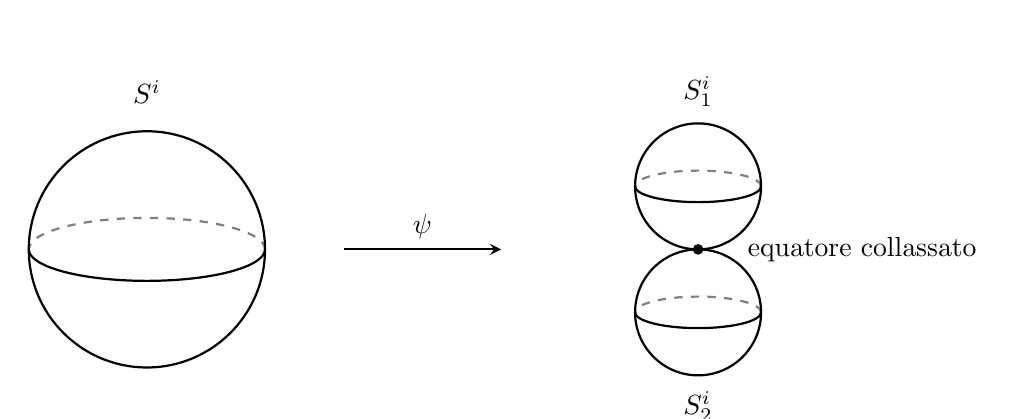
\begin{tikzpicture}[>=stealth, thick]
        % Sfera originale S^i
        \draw (0,0) circle (1.5);
        % Equatore (davanti e dietro)
        \draw (-1.5,0) arc (180:360:1.5 and 0.4);
        \draw[dashed, opacity=0.5] (1.5,0) arc (0:180:1.5 and 0.4);
        \node at (0, 2) {$S^i$};
        
        % Freccia della mappa
        \draw[->] (2.5,0) -- (4.5,0) node[midway, above] {$\psi$};
        
        % Sfera quozientata (Wedge sum S^i_1 \vee S^i_2)
        \begin{scope}[shift={(7,0)}]
            % Sfera superiore
            \draw (0, 0.8) circle (0.8);
            \draw (-0.8, 0.8) arc (180:360:0.8 and 0.2);
            \draw[dashed, opacity=0.5] (0.8, 0.8) arc (0:180:0.8 and 0.2);
            \node at (0, 2) {$S^i_1$};
            
            % Sfera inferiore
            \draw (0, -0.8) circle (0.8);
            \draw (-0.8, -0.8) arc (180:360:0.8 and 0.2);
            \draw[dashed, opacity=0.5] (0.8, -0.8) arc (0:180:0.8 and 0.2);
            \node at (0, -2) {$S^i_2$};
            
            % Punto di incollaggio (equatore collassato)
            \filldraw (0,0) circle (1.5pt) node[right, xshift=5mm] {equatore collassato};
        \end{scope}
    \end{tikzpicture}
    \caption{La mappa $\psi$ che collassa l'equatore della sfera $S^i$.}
\end{figure}
Effettuare le dimostrazioni (come l'associatività e l'esistenza dell'inverso) direttamente su una sfera è abbastanza \emph{tricky} e complicato per via della geometria dei domini. Per semplificare enormemente la costruzione, si usa il fatto che $D^i$ è omeomorfo al cubo $[-1, 1]^i$ (o, a meno di traslazioni, a $[0,1]^i$)\footnote{Un quadrato è omeomorfo alla palla chiusa, ovvero sono topologicamente equivalenti. È abbastanza semplice far vedere questo poiché,
preso un punto su una palla, posso considerare $f: D^i \to [-1,1]^i$ definita nel seguente modo:
\begin{align}
    f(x) = \begin{cases}
        x\frac{||x||_2}{||x||_{\infty}} & \text{se } x \neq 0 \\
        0 & \text{se } x = 0
    \end{cases},
\end{align}
dove $||x||_\infty = \max_i{|x_i|}$ ed è facile far vedere che questa funzione è continua rispetto a $||\cdot||_{\infty}$ (infatti la topologia sul quadrato è quella data dalla norma del massimo, quindi devo mostrare la continuità con quella) in $x=0$ poiché
\begin{align}
    ||f(x) - f(0)||_{\infty} = ||f(x)||_{\infty} = \left|\left|x\frac{||x||_2}{||x||_{\infty}}\right|\right|_{\infty} = ||x||_{\infty} \frac{||x||_2}{||x||_\infty} = ||x||_2 \to 0 \text{ per } x \to 0,
\end{align}
e il mapping inverso $f^{-1}: [-1, 1]^i \to D^i$ è dato da:
\begin{align}
    f^{-1}(z) = \begin{cases}
        z \frac{||z||_{\infty}}{||z||_2} & \text{se } z \neq 0 \\
        0 & \text{se } z = 0.
    \end{cases},
\end{align}
e possiamo procedere similmente a quanto fatto sopra per la continuità di $f$ per mostrare che anche $f^{-1}$ è continua. Per quanto riguarda la bigettività, osserviamo che
\begin{align}
    (f \circ f^{-1})(z) = f\left(z \frac{||z||_{\infty}}{||z||_2}\right) = z \frac{||z||_{\infty}}{||z||_2} \frac{\left|\left|z \frac{||z||_{\infty}}{||z||_{2}}\right|\right|_{2}}{\left|\left| z \frac{||z||_{\infty}}{||z||_{2}} \right|\right|_\infty} = z,
\end{align}
dunque $f \circ f^{-1} = \id_{[-1, 1]^i}$ e similmente si procede per vedere che $f^{-1} \circ f = \id_{D^i}$.
}.
 
Lavorando sul dominio a coordinate $I^i = I^{i-1} \times [0,1]$, indicando un punto generico con $(x, s)$ dove $x \in I^{i-1}$ e $s \in [0,1]$, il prodotto di due mappe $\alpha, \beta \in \pi_i(X)$ è così definito:
\begin{align}
    (\alpha \circ \beta)(x, s) = \begin{cases}
        \alpha(x, 2s) & \text{se } 0 \leq s \leq \frac{1}{2} \\
        \beta(x, 2s-1) & \text{se } \frac{1}{2} < s \leq 1
    \end{cases}.
\end{align}

Siamo pronti per mostrare che questo spazio ha la struttura di gruppo: cercherò per quanto possibile di rifarmi alla definizione "sferica" del concetto (che Konishi ha usato in classe), ma per l'associatività sarò costretto ad andare nel cubo $i-$dimensionale.
\begin{theorem}
    Sia $X$ uno spazio topologico (o una varietà) e sia $\pi_j(X, x_0)$ il gruppo $j$-esimo di omotopia con $j \geq 2$. Se indichiamo con $\psi: S^i \to S^i_1 \vee S^i_2$ la mappa di schiacciamento spiegata sopra, l'emisfero positivo $D^+=\{(x^0, \ldots, x^{i}) \in \mathbb{R}^{i+1}: (x^0)^2 + \ldots + (x^i)^2 = 1, x^0 \geq 0 \}$, l'emisfero negativo $D^-=\{ (x^0, \ldots, x^{i}) \in \mathbb{R}^{i+1}: (x^0)^2 + \ldots + (x^i)^2 = 1, x^0 \leq 0 \}$ e definiamo il prodotto di mappe $\alpha, \beta \in \pi_j(X, x_0)$ come
    \begin{align}
        (\alpha \cdot \beta)(x) = \begin{cases}
            \alpha(\psi(x)) & \text{se } x \in D^+, \\
            \beta(\psi(x)) & \text{se } x \in D^-
        \end{cases},
    \end{align} 
    allora:
    \begin{enumerate}[label=\protect\circled{\arabic*}]
        \item $\pi_j(X, x_0)$ è un gruppo rispetto a $\cdot$;
        \item $\pi_j(X, x_0)$ è un gruppo abeliano. 
    \end{enumerate}
\end{theorem}
\begin{proof}
    Mostriamo la $\circled{1}$: per farlo è necessario mostrare l'associatività, l'esistenza dell'elemento neutro e l'esistenza dell'elemento inverso. 
    
    \textbf{Associatività:} Possiamo immaginare che $D^-$ sia separato a sua volta in due regioni: $D^- = D^-_1 \cup D^-_2$ con $x^1 \leq 0$ in $D^-_1$ e $x^1 \geq 0$ in $D^-_2$. Possiamo quindi definire una mappa $\tilde{\psi}$ che collassa in un singolo punto $s_0$ sia l'equatore sia il semicerchio che separa $D^-_1$ e $D^-_2$, ottenendo una struttura "a trifoglio". Con questo modello geometrico, l'omotopia che manda $\alpha \cdot (\beta \cdot \gamma)$ in $(\alpha \cdot \beta) \cdot \gamma$ corrisponde a far scivolare con continuità i "muri" di separazione sulla sfera originale.
    
    \begin{figure}[htbp]
    \centering
    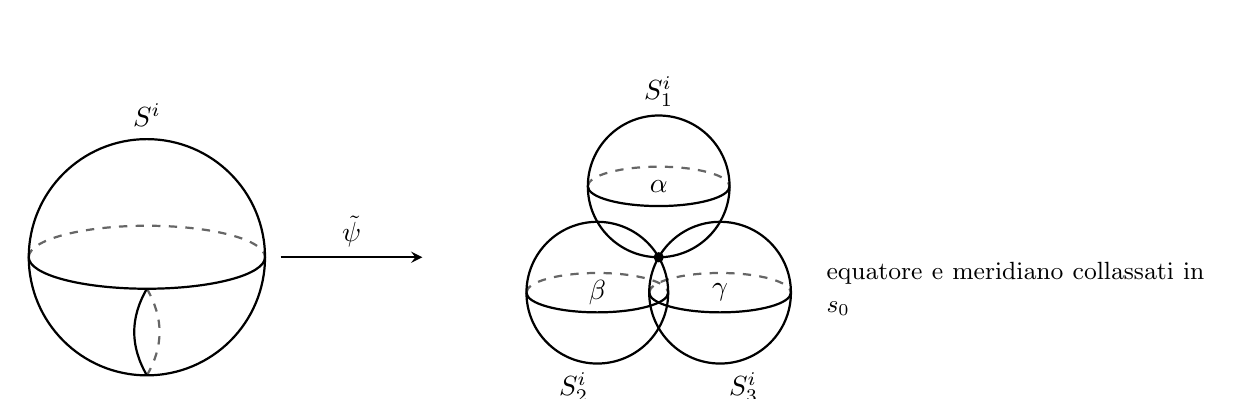
\begin{tikzpicture}[>=stealth, thick]
      \tikzset{dashed line/.style={dashed, opacity=0.6}}
      \tikzset{solid line/.style={solid}}

      \begin{scope}[shift={(-2.5, 0)}]
        \draw (0, 0) circle (1.5);
        \node at (0, 1.8) {\(S^i\)};
        \draw[dashed line] (-1.5, 0) arc (180:0:1.5 and 0.4);
        \draw[solid line] (1.5, 0) arc (0:-180:1.5 and 0.4);
        \draw[solid line] (0, -0.4) to[bend right=30] (0, -1.5);
        \draw[dashed line] (0, -0.4) to[bend left=30] (0, -1.5);
      \end{scope}

      \draw[->] (-0.8, 0) -- (1.0, 0) node[midway, above] {\(\tilde{\psi}\)};

      \begin{scope}[shift={(4, 0)}]
        \def\rsmall{0.9}
        \def\rcos{0.7794}
        \def\rsin{0.45}
        \coordinate (C1) at (0, \rsmall);
        \coordinate (C2) at (-\rcos, -\rsin);
        \coordinate (C3) at (\rcos, -\rsin);

        \begin{scope}[shift={(C1)}]
          \draw circle (\rsmall);
          \node at (0, \rsmall + 0.3) {\(S^i_1\)};
          \node at (0, 0) {\(\alpha\)};
          \draw[dashed line] (-\rsmall, 0) arc (180:0:{\rsmall} and 0.25);
          \draw[solid line] (\rsmall, 0) arc (0:-180:{\rsmall} and 0.25);
        \end{scope}

        \begin{scope}[shift={(C2)}]
          \draw circle (\rsmall);
          \node at (-0.3, -\rsmall - 0.3) {\(S^i_2\)};
          \node at (0, 0) {\(\beta\)};
          \draw[dashed line] (-\rsmall, 0) arc (180:0:{\rsmall} and 0.25);
          \draw[solid line] (\rsmall, 0) arc (0:-180:{\rsmall} and 0.25);
        \end{scope}

        \begin{scope}[shift={(C3)}]
          \draw circle (\rsmall);
          \node at (0.3, -\rsmall - 0.3) {\(S^i_3\)};
          \node at (0, 0) {\(\gamma\)};
          \draw[dashed line] (-\rsmall, 0) arc (180:0:{\rsmall} and 0.25);
          \draw[solid line] (\rsmall, 0) arc (0:-180:{\rsmall} and 0.25);
        \end{scope}

        \draw[fill=black, thick] (0, 0) circle (0.05);
        \node[right, xshift=20mm, yshift=-4mm, text width=5cm, align=left] at (0,0) {\small equatore e meridiano collassati in \(s_0\)};
      \end{scope}
    \end{tikzpicture}
    \caption{Trifoglio topologico generato dalla mappa di schiacciamento potenziata $\tilde{\psi}$.}
    \end{figure}

    Per scrivere in modo esplicito l'omotopia dell'associatività in termini puramente algebrici, è d'uso parametrizzare l'operazione tramite la coordinata di concatenazione $s \in [0,1]$ (che equivale a lavorare su un cubo che su una sfera). L'omotopia $H(x, s, t)$ muove i confini temporali dei tre raggruppamenti:
    \begin{align}
        H(x, s, t) = \begin{cases}
            \alpha\left(x, \, \frac{4s}{2-t}\right) & \text{se } 0 \leq s \leq \frac{2-t}{4} \\[8pt]
            \beta\Big(x, \, 4s - 2 + t\Big) & \text{se } \frac{2-t}{4} \leq s \leq \frac{3-t}{4} \\[8pt]
            \gamma\left(x, \, \frac{4s - 3 + t}{1+t}\right) & \text{se } \frac{3-t}{4} \leq s \leq 1
        \end{cases}
    \end{align}
    A $t=0$ questa formula restituisce esattamente $\alpha \cdot (\beta \cdot \gamma)$, mentre a $t=1$ restituisce $(\alpha \cdot \beta) \cdot \gamma$, garantendo l'incollatura nei punti di separazione per ogni $t$.

    \textbf{Elemento neutro:} Mostriamo che $\alpha \cdot f \sim c_{x_0} \cdot f$, dove $\alpha$ è omotopa alla funzione costante $c_{x_0}$. L'omotopia esplicita può essere scritta facilmente utilizzando la mappa $\psi: S^i \to S^i_1 \vee S^i_2$ nel seguente modo:
    \begin{align}
        H(x, t) = \begin{cases}
            C(\psi(x), t) & \text{se } \psi(x) \in S^i_1 \\
            f(\psi(x)) & \text{se } \psi(x) \in S^i_2
        \end{cases},
    \end{align}
    dove $C: S^i \times [0,1] \to X$ è l'omotopia garantita dal fatto che $\alpha \sim c_{x_0}$, tale che $C(y, 0) = \alpha(y)$ e $C(y, 1) = x_0$. Chiaramente, al tempo $t=0$ otteniamo $H(x, 0) = (\alpha \cdot f)(x)$, mentre al tempo $t=1$ l'intera palla superiore è mappata in $x_0$, restituendo $H(x, 1) = (c_{x_0} \cdot f)(x)$. Di conseguenza $\alpha \cdot f \sim c_{x_0} \cdot f$. 
    
    Resta da mostrare che $c_{x_0} \cdot f \sim f$. Geometricamente, sul dominio sferico $S^i$, la mappa $c_{x_0} \cdot f$ è costantemente uguale a $x_0$ sull'emisfero nord, ed equivale alla mappa $f$ sull'emisfero sud. L'omotopia tra questa mappa e $f$ consiste nel far "scivolare" l'equatore in modo continuo verso il Polo Nord. Utilizzando nuovamente la coordinata di parametrizzazione $s \in [0,1]$, l'omotopia esplicita che dilata il dominio di $f$ fino a fargli occupare tutto lo spazio è:
    \begin{align}
        K(x, s, t) = \begin{cases}
            x_0 & \text{se } 0 \leq s \leq \frac{1-t}{2} \\[6pt]
            f\left(x, \, \frac{2s - 1 + t}{1+t}\right) & \text{se } \frac{1-t}{2} \leq s \leq 1
        \end{cases}
    \end{align}
    Al tempo $t=0$, $K$ vale $c_{x_0} \cdot f$, mentre al tempo $t=1$ il termine di separazione collassa a $0$ e l'espressione diventa $K(x, s, 1) = f(x, s)$. Questo dimostra rigorosamente che $[c_{x_0} \cdot f] = [f]$.

    \textbf{Elemento inverso:} Posso considerare la mappa $(x^0, \ldots, x^i) \stackrel{\bar{\alpha}}{\mapsto} \alpha(-x^0, \ldots, x^i)$ ed osservare che in questa maniera:
    \begin{align}
        (\alpha \cdot \bar{\alpha})(x^0, \ldots, x^i) = \begin{cases}
            \alpha(x^0, \ldots, x^i) & \text{se } x^0 \geq 0 \\
            \alpha(-x^0, \ldots, x^i) & \text{se } x^0 < 0
        \end{cases}
    \end{align}
    Questa costruzione fa in modo che i punti $x = (x^0, \ldots, x^i)$ e $x^* = (-x^0, \ldots, x^i)$ vengano mappati nello stesso valore. Si ha quindi $\alpha \cdot \bar{\alpha} = \alpha \cdot \pi$, con $\pi: S^i \to D^i$ che è la proiezione che schiaccia la sfera sul disco equatoriale. Poiché $D^i$ è uno spazio contraibile, per il teorema introdotto precedentemente la composizione $\alpha \cdot \pi$ è omotopa alla mappa costante $c_{x_0}$. \newline

    Mostriamo infine la $\circled{2}$: per farlo osserviamo che una rotazione continua attorno al complemento ortogonale del piano $(x_0, x_1)$ scambia con continuità $D^+$ con $D^-$. Questo movimento definisce l'omotopia desiderata, dimostrando che $\alpha \cdot \beta \sim \beta \cdot \alpha$.
\end{proof}

	\newpage
	\pagebreak
	\newpage
	\clearpage
	\cleardoublepage
	\pagestyle{plain}
	\thispagestyle{empty}
	\pagestyle{empty}
	\appendix
	
	\fancyhead[LO]{\textbf{\thepage}}  % Numero di pagina in grassetto a sinistra
	\fancyhead[RO]{\nouppercase\rightmark}         % Capitolo e sezione a destra

	% Definizione dell'intestazione per pagine pari (Even)
	\fancyhead[LE]{\nouppercase\leftmark}          % Capitolo e sezione a sinistra
	\fancyhead[RE]{\textbf{\thepage}}  % Numero di pagina in grassetto a destra

		% Cancella il footer
	\fancyfoot{}
	\setlength{\headheight}{14.49998pt}
	\addtolength{\topmargin}{-2.49998pt}
	% Personalizzazione della linea orizzontale
	\renewcommand{\headrulewidth}{0.4pt}
	\renewcommand{\footrulewidth}{0pt}
	\vspace*{\fill}
	\begin{figure}[H]
		\centering
		\hspace*{-1cm}
	
\includegraphics[scale=1.80]{immagini/xi_graphic.png}
	\end{figure}
	\vspace*{\fill}
	\clearpage
	\cleardoublepage
		\pagestyle{fancy}
		\include{capitoli/logica}
		\include{capitoli/basi_dimensione_infinita}
	\cleardoublepage
	\addcontentsline{toc}{chapter}{Bibliografia}
	\bibliographystyle{unsrt}
	\bibliography{bibliography.bib}
\end{document}
